% Options for packages loaded elsewhere
\PassOptionsToPackage{unicode}{hyperref}
\PassOptionsToPackage{hyphens}{url}
\PassOptionsToPackage{dvipsnames,svgnames,x11names}{xcolor}
%
\documentclass[
  11pt,
]{krantz}
\usepackage{amsmath,amssymb}
\usepackage{lmodern}
\usepackage{iftex}
\ifPDFTeX
  \usepackage[T1]{fontenc}
  \usepackage[utf8]{inputenc}
  \usepackage{textcomp} % provide euro and other symbols
\else % if luatex or xetex
  \usepackage{unicode-math}
  \defaultfontfeatures{Scale=MatchLowercase}
  \defaultfontfeatures[\rmfamily]{Ligatures=TeX,Scale=1}
  \setmonofont[Scale=0.775]{MesloLGS NF}
\fi
% Use upquote if available, for straight quotes in verbatim environments
\IfFileExists{upquote.sty}{\usepackage{upquote}}{}
\IfFileExists{microtype.sty}{% use microtype if available
  \usepackage[]{microtype}
  \UseMicrotypeSet[protrusion]{basicmath} % disable protrusion for tt fonts
}{}
\makeatletter
\@ifundefined{KOMAClassName}{% if non-KOMA class
  \IfFileExists{parskip.sty}{%
    \usepackage{parskip}
  }{% else
    \setlength{\parindent}{0pt}
    \setlength{\parskip}{6pt plus 2pt minus 1pt}}
}{% if KOMA class
  \KOMAoptions{parskip=half}}
\makeatother
\usepackage{xcolor}
\IfFileExists{xurl.sty}{\usepackage{xurl}}{} % add URL line breaks if available
\IfFileExists{bookmark.sty}{\usepackage{bookmark}}{\usepackage{hyperref}}
\hypersetup{
  pdftitle={Data Science per psicologi},
  pdfauthor={Corrado Caudek},
  colorlinks=true,
  linkcolor={Maroon},
  filecolor={Maroon},
  citecolor={Blue},
  urlcolor={Blue},
  pdfcreator={LaTeX via pandoc}}
\urlstyle{same} % disable monospaced font for URLs
\usepackage{color}
\usepackage{fancyvrb}
\newcommand{\VerbBar}{|}
\newcommand{\VERB}{\Verb[commandchars=\\\{\}]}
\DefineVerbatimEnvironment{Highlighting}{Verbatim}{commandchars=\\\{\}}
% Add ',fontsize=\small' for more characters per line
\usepackage{framed}
\definecolor{shadecolor}{RGB}{248,248,248}
\newenvironment{Shaded}{\begin{snugshade}}{\end{snugshade}}
\newcommand{\AlertTok}[1]{\textcolor[rgb]{0.33,0.33,0.33}{#1}}
\newcommand{\AnnotationTok}[1]{\textcolor[rgb]{0.37,0.37,0.37}{\textbf{\textit{#1}}}}
\newcommand{\AttributeTok}[1]{\textcolor[rgb]{0.61,0.61,0.61}{#1}}
\newcommand{\BaseNTok}[1]{\textcolor[rgb]{0.06,0.06,0.06}{#1}}
\newcommand{\BuiltInTok}[1]{#1}
\newcommand{\CharTok}[1]{\textcolor[rgb]{0.5,0.5,0.5}{#1}}
\newcommand{\CommentTok}[1]{\textcolor[rgb]{0.37,0.37,0.37}{\textit{#1}}}
\newcommand{\CommentVarTok}[1]{\textcolor[rgb]{0.37,0.37,0.37}{\textbf{\textit{#1}}}}
\newcommand{\ConstantTok}[1]{\textcolor[rgb]{0,0,0}{#1}}
\newcommand{\ControlFlowTok}[1]{\textcolor[rgb]{0.27,0.27,0.27}{\textbf{#1}}}
\newcommand{\DataTypeTok}[1]{\textcolor[rgb]{0.27,0.27,0.27}{#1}}
\newcommand{\DecValTok}[1]{\textcolor[rgb]{0.06,0.06,0.06}{#1}}
\newcommand{\DocumentationTok}[1]{\textcolor[rgb]{0.37,0.37,0.37}{\textbf{\textit{#1}}}}
\newcommand{\ErrorTok}[1]{\textcolor[rgb]{0.14,0.14,0.14}{\textbf{#1}}}
\newcommand{\ExtensionTok}[1]{#1}
\newcommand{\FloatTok}[1]{\textcolor[rgb]{0.06,0.06,0.06}{#1}}
\newcommand{\FunctionTok}[1]{\textcolor[rgb]{0,0,0}{#1}}
\newcommand{\ImportTok}[1]{#1}
\newcommand{\InformationTok}[1]{\textcolor[rgb]{0.37,0.37,0.37}{\textbf{\textit{#1}}}}
\newcommand{\KeywordTok}[1]{\textcolor[rgb]{0.27,0.27,0.27}{\textbf{#1}}}
\newcommand{\NormalTok}[1]{#1}
\newcommand{\OperatorTok}[1]{\textcolor[rgb]{0.43,0.43,0.43}{\textbf{#1}}}
\newcommand{\OtherTok}[1]{\textcolor[rgb]{0.37,0.37,0.37}{#1}}
\newcommand{\PreprocessorTok}[1]{\textcolor[rgb]{0.37,0.37,0.37}{\textit{#1}}}
\newcommand{\RegionMarkerTok}[1]{#1}
\newcommand{\SpecialCharTok}[1]{\textcolor[rgb]{0,0,0}{#1}}
\newcommand{\SpecialStringTok}[1]{\textcolor[rgb]{0.5,0.5,0.5}{#1}}
\newcommand{\StringTok}[1]{\textcolor[rgb]{0.5,0.5,0.5}{#1}}
\newcommand{\VariableTok}[1]{\textcolor[rgb]{0,0,0}{#1}}
\newcommand{\VerbatimStringTok}[1]{\textcolor[rgb]{0.5,0.5,0.5}{#1}}
\newcommand{\WarningTok}[1]{\textcolor[rgb]{0.37,0.37,0.37}{\textbf{\textit{#1}}}}
\usepackage{longtable,booktabs,array}
\usepackage{calc} % for calculating minipage widths
% Correct order of tables after \paragraph or \subparagraph
\usepackage{etoolbox}
\makeatletter
\patchcmd\longtable{\par}{\if@noskipsec\mbox{}\fi\par}{}{}
\makeatother
% Allow footnotes in longtable head/foot
\IfFileExists{footnotehyper.sty}{\usepackage{footnotehyper}}{\usepackage{footnote}}
\makesavenoteenv{longtable}
\usepackage{graphicx}
\makeatletter
\def\maxwidth{\ifdim\Gin@nat@width>\linewidth\linewidth\else\Gin@nat@width\fi}
\def\maxheight{\ifdim\Gin@nat@height>\textheight\textheight\else\Gin@nat@height\fi}
\makeatother
% Scale images if necessary, so that they will not overflow the page
% margins by default, and it is still possible to overwrite the defaults
% using explicit options in \includegraphics[width, height, ...]{}
\setkeys{Gin}{width=\maxwidth,height=\maxheight,keepaspectratio}
% Set default figure placement to htbp
\makeatletter
\def\fps@figure{htbp}
\makeatother
\setlength{\emergencystretch}{3em} % prevent overfull lines
\providecommand{\tightlist}{%
  \setlength{\itemsep}{0pt}\setlength{\parskip}{0pt}}
\setcounter{secnumdepth}{5}
\usepackage{amsmath}
\usepackage{amssymb}
\usepackage{amsfonts}

\defaultfontfeatures{Scale=MatchLowercase}

\usepackage{booktabs}
\usepackage{longtable}
\usepackage[bf,singlelinecheck=off]{caption}

\usepackage{framed,color}
\definecolor{shadecolor}{RGB}{248,248,248}

\renewcommand{\textfraction}{0.05}
\renewcommand{\topfraction}{0.8}
\renewcommand{\bottomfraction}{0.8}
\renewcommand{\floatpagefraction}{0.75}

\renewenvironment{quote}{\begin{VF}}{\end{VF}}
\let\oldhref\href
\renewcommand{\href}[2]{#2\footnote{\url{#1}}}

\ifxetex
  \usepackage{letltxmacro}
  \setlength{\XeTeXLinkMargin}{1pt}
  \LetLtxMacro\SavedIncludeGraphics\includegraphics
  \def\includegraphics#1#{% #1 catches optional stuff (star/opt. arg.)
    \IncludeGraphicsAux{#1}%
  }%
  \newcommand*{\IncludeGraphicsAux}[2]{%
    \XeTeXLinkBox{%
      \SavedIncludeGraphics#1{#2}%
    }%
  }%
\fi

\makeatletter
\newenvironment{kframe}{%
\medskip{}
\setlength{\fboxsep}{.8em}
 \def\at@end@of@kframe{}%
 \ifinner\ifhmode%
  \def\at@end@of@kframe{\end{minipage}}%
  \begin{minipage}{\columnwidth}%
 \fi\fi%
 \def\FrameCommand##1{\hskip\@totalleftmargin \hskip-\fboxsep
 \colorbox{shadecolor}{##1}\hskip-\fboxsep
     % There is no \\@totalrightmargin, so:
     \hskip-\linewidth \hskip-\@totalleftmargin \hskip\columnwidth}%
 \MakeFramed {\advance\hsize-\width
   \@totalleftmargin\z@ \linewidth\hsize
   \@setminipage}}%
 {\par\unskip\endMakeFramed%
 \at@end@of@kframe}
\makeatother

\renewenvironment{Shaded}{\begin{kframe}}{\end{kframe}}

\usepackage{makeidx}
\makeindex

\urlstyle{tt}

\usepackage{amsthm}
\makeatletter
\def\thm@space@setup{%
  \thm@preskip=8pt plus 2pt minus 4pt
  \thm@postskip=\thm@preskip
}
\makeatother

\DeclareMathOperator{\V}{\mathbb{V}} % Define variance operator
\DeclareMathOperator{\Var}{\mathbb{V}} % Define variance operator
\DeclareMathOperator{\SD}{SD} % Define sd operator
\DeclareMathOperator{\Cov}{Cov} % Define covariance operator
\DeclareMathOperator{\Corr}{Corr} % Define correlation operator
\DeclareMathOperator{\Me}{Me} % Define mediane operator
\DeclareMathOperator{\Mo}{Mo} % Define mode operator

\DeclareMathOperator{\Bin}{Binomial} % Define binomial operator
\DeclareMathOperator{\Bernoulli}{Bernoulli} % Define Bernoulli operator
\DeclareMathOperator{\Ber}{\mathscr{B}} % Define Bernoulli operator
\DeclareMathOperator{\Poi}{Poisson} % Define Poisson operator
\DeclareMathOperator{\Uniform}{Uniform} % Define Uniform operator
\DeclareMathOperator{\Cauchy}{Cauchy} % Define Cauchy operator
\DeclareMathOperator{\B}{B} % beta function
% \mbox{B}(a, b) % beta function
% \mbox{Beta}(a, b) % beta distribution

\DeclareMathOperator{\elpd}{elpd} % Define elpd operator
\DeclareMathOperator{\lppd}{lppd} % Define lppd operator
\DeclareMathOperator{\LOO}{LOO} % Define LOO operator
\DeclareMathOperator{\argmin}{arg\,min} 
\DeclareMathOperator{\argmax}{arg\,max} 

\newcommand{\E}{\mathbb{E}} % Define expected value operator
\newcommand{\R}{\textsf{R}} % Define R programming language symbol
\newcommand{\Real}{\mathbb{R}} % Define real number operator
\newcommand{\Prob}{\mathscr{P}}
\newcommand{\indep}{\perp \!\!\! \perp}

\usepackage[
 labelfont=bf,
 font={small, it}
]{caption}
\usepackage{upquote} % print correct quotes in verbatim-environments
\usepackage{empheq}
\usepackage{xfrac}

\usepackage{polyglossia}
\setmainlanguage{italian}

\frontmatter
\ifLuaTeX
  \usepackage{selnolig}  % disable illegal ligatures
\fi
\usepackage[]{natbib}
\bibliographystyle{apalike}

\title{Data Science per psicologi}
\author{Corrado Caudek}
\date{2022-02-12}

\usepackage{amsthm}
\newtheorem{theorem}{Teorema}[chapter]
\newtheorem{lemma}{Lemma}[chapter]
\newtheorem{corollary}{Corollario}[chapter]
\newtheorem{proposition}{Proposizione}[chapter]
\newtheorem{conjecture}{Congettura}[chapter]
\theoremstyle{definition}
\newtheorem{definition}{Definizione}[chapter]
\theoremstyle{definition}
\newtheorem{example}{Esempio}[chapter]
\theoremstyle{definition}
\newtheorem{exercise}{Esercizio}[chapter]
\theoremstyle{definition}
\newtheorem{hypothesis}{Hypothesis}[chapter]
\theoremstyle{remark}
\newtheorem*{remark}{Osservazione}
\newtheorem*{solution}{Soluzione}
\begin{document}
\maketitle

\cleardoublepage\newpage\thispagestyle{empty}\null
% \cleardoublepage\newpage\thispagestyle{empty}\null
%\cleardoublepage\newpage
\thispagestyle{empty}
\begin{center}
\Large{Psicometria -- AA 2021/2022}

\vskip20pt

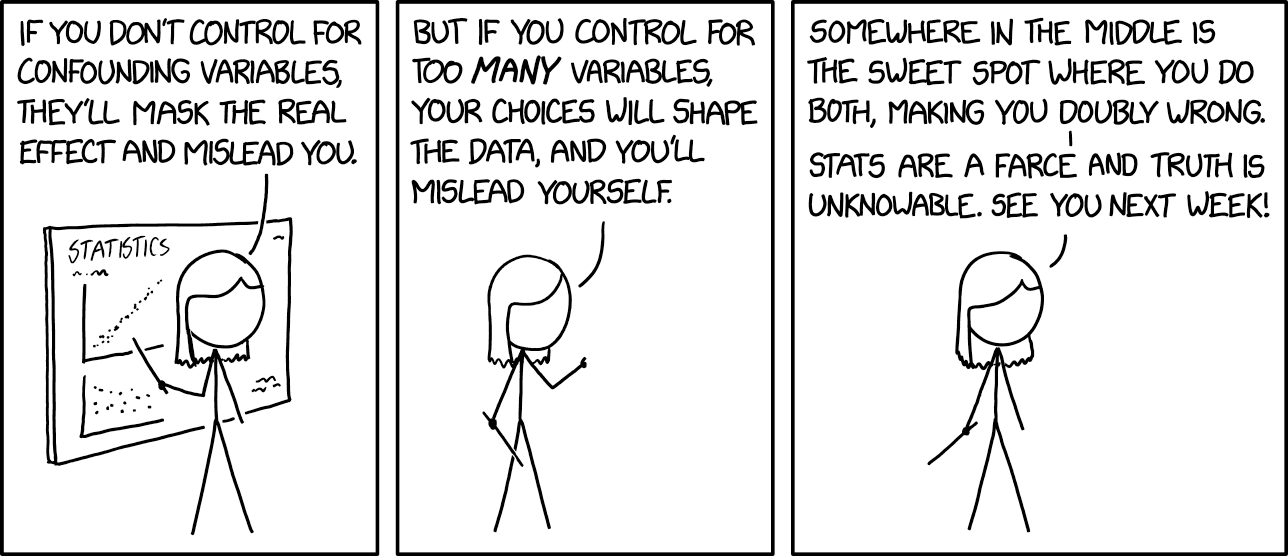
\includegraphics{images/confounding_variables.png}
\end{center}

\setlength{\abovedisplayskip}{-5pt}
\setlength{\abovedisplayshortskip}{-5pt}

{
\hypersetup{linkcolor=}
\setcounter{tocdepth}{2}
\tableofcontents
}
\listoffigures
\listoftables
\hypertarget{prefazione}{%
\chapter*{Prefazione}\label{prefazione}}


\emph{Data Science per psicologi} contiene il materiale delle lezioni dell'insegnamento di \emph{Psicometria B000286} (A.A. 2021/2022) rivolto agli studenti del primo anno del Corso di Laurea in Scienze e Tecniche Psicologiche dell'Università degli Studi di Firenze. \emph{Psicometria} si propone di fornire agli studenti un'introduzione all'analisi dei dati in psicologia. Le conoscenze/competenze che verranno sviluppate in questo insegnamento sono quelle della Data science, ovvero un insieme di conoscenze/competenze che si pongono all'intersezione tra statistica (ovvero, richiedono la capacità di comprendere teoremi statistici) e informatica (ovvero, richiedono la capacità di sapere utilizzare un software).

\hypertarget{la-psicologia-e-la-data-science}{%
\section*{La psicologia e la Data science}\label{la-psicologia-e-la-data-science}}


Sembra sensato spendere due parole su un tema che è importante per gli studenti: quello indicato dal titolo di questo Capitolo. È ovvio che agli studenti di psicologia la statistica non piace. Se piacesse, forse studierebbero Data science e non psicologia; ma non lo fanno. Di conseguenza, gli studenti di psicologia si chiedono: ``perché dobbiamo perdere tanto tempo a studiare queste cose quando in realtà quello che ci interessa è tutt'altro?'' Questa è una bella domanda.

C'è una ragione molto semplice che dovrebbe farci capire perché la Data science è così importante per la psicologia. Infatti, a ben pensarci, la psicologia è una disciplina intrinsecamente statistica, se per statistica intendiamo quella disciplina che studia la variazione delle caratteristiche degli individui nella popolazione. La psicologia studia \emph{gli individui} ed è proprio la variabilità inter- e intra-individuale ciò che vogliamo descrivere e, in certi casi, predire. In questo senso, la psicologia è molto diversa dall'ingegneria, per esempio. Le proprietà di un determinato ponte sotto certe condizioni, ad esempio, sono molto simili a quelle di un altro ponte, sotto le medesime condizioni. Quindi, per un ingegnere la statistica è poco importante: le proprietà dei materiali sono unicamente dipendenti dalla loro composizione e restano costanti. Ma lo stesso non può dirsi degli individui: ogni individuo è unico e cambia nel tempo. E le variazioni tra gli individui, e di un individuo nel tempo, sono l'oggetto di studio proprio della psicologia: è dunque chiaro che i problemi che la psicologia si pone sono molto diversi da quelli affrontati, per esempio, dagli ingegneri. Questa è la ragione per cui abbiamo tanto bisogno della Data science in psicologia: perché la Data science ci consente di descrivere la variazione e il cambiamento. E queste sono appunto le caratteristiche di base dei fenomeni psicologici.

Sono sicuro che, leggendo queste righe, a molti studenti sarà venuta in mente la seguente domanda: perché non chiediamo a qualche esperto di fare il ``lavoro sporco'' (ovvero le analisi statistiche) per noi, mentre noi (gli psicologi) ci occupiamo solo di ciò che ci interessa, ovvero dei problemi psicologici slegati dai dettagli ``tecnici'' della Data science? La risposta a questa domanda è che non è possibile progettare uno studio psicologico sensato senza avere almeno una comprensione rudimentale della Data science. Le tematiche della Data science non possono essere ignorate né dai ricercatori in psicologia né da coloro che svolgono la professione di psicologo al di fuori dell'Università. Infatti, anche i professionisti al di fuori dall'università non possono fare a meno di leggere la letteratura psicologica più recente: il continuo aggiornamento delle conoscenze è infatti richiesto dalla deontologia della professione. Ma per potere fare questo è necessario conoscere un bel po' di Data science! Basta aprire a caso una rivista specialistica di psicologia per rendersi conto di quanto ciò sia vero: gli articoli che riportano i risultati delle ricerche psicologiche sono zeppi di analisi statistiche e di modelli formali. E la comprensione della letteratura psicologica rappresenta un requisito minimo nel bagaglio professionale dello psicologo.

Le considerazioni precedenti cercano di chiarire il seguente punto: la Data science non è qualcosa da studiare a malincuore, in un singolo insegnamento universitario, per poi poterla tranquillamente dimenticare. Nel bene e nel male, gli psicologi usano gli strumenti della Data science in tantissimi ambiti della loro attività professionale: in particolare quando costruiscono, somministrano e interpretano i test psicometrici. È dunque chiaro che possedere delle solide basi di Data science è un tassello imprescindibile del bagaglio professionale dello psicologo. In questo insegnamento verrano trattati i temi base della Data science e verrà adottato un punto di vista bayesiano, che corrisponde all'approccio più recente e sempre più diffuso in psicologia.

\hypertarget{come-studiare}{%
\section*{Come studiare}\label{come-studiare}}


Il giusto metodo di studio per prepararsi all'esame di Psicometria è quello di seguire attivamente le lezioni, assimilare i concetti via via che essi vengono presentati e verificare in autonomia le procedure presentate a lezione. Incoraggio gli studenti a farmi domande per chiarire ciò che non è stato capito appieno. Incoraggio gli studenti a utilizzare i forum attivi su Moodle e, soprattutto, a svolgere gli esercizi proposti su Moodle. I problemi forniti su Moodle rappresentano il livello di difficoltà richiesto per superare l'esame e consentono allo studente di comprendere se le competenze sviluppate fino a quel punto sono sufficienti rispetto alle richieste dell'esame.

La prima fase dello studio, che è sicuramente individuale, è quella in cui è necessario acquisire le conoscenze teoriche relative ai problemi che saranno presentati all'esame. La seconda fase di studio, che può essere facilitata da scambi con altri e da incontri di gruppo, porta ad acquisire la capacità di applicare le conoscenze: è necessario capire come usare un software (\(\textsf{R}\)) per applicare i concetti statistici alla specifica situazione del problema che si vuole risolvere. Le due fasi non sono però separate: il saper fare molto spesso ci aiuta a capire meglio.

\hypertarget{sviluppare-un-metodo-di-studio-efficace}{%
\section*{Sviluppare un metodo di studio efficace}\label{sviluppare-un-metodo-di-studio-efficace}}


Avendo insegnato molte volte in passato un corso introduttivo di analisi dei dati ho notato nel corso degli anni che gli studenti con l'atteggiamento mentale che descriverò qui sotto generalmente ottengono ottimi risultati. Alcuni studenti sviluppano naturalmente questo approccio allo studio, ma altri hanno bisogno di fare uno sforzo per maturarlo. Fornisco qui sotto una breve descrizione del ``metodo di studio'' che, nella mia esperienza, è il più efficace per affrontare le richieste di questo insegnamento.

\begin{itemize}
\tightlist
\item
  Dedicate un tempo sufficiente al materiale di base, apparentemente facile; assicuratevi di averlo capito bene. Cercate le lacune nella vostra comprensione. Leggere presentazioni diverse dello stesso materiale (in libri o articoli diversi) può fornire nuove intuizioni.
\item
  Gli errori che facciamo sono i nostri migliori maestri. Istintivamente cerchiamo di dimenticare subito i nostri errori. Ma il miglior modo di imparare è apprendere dagli errori che commettiamo. In questo senso, una soluzione corretta è meno utile di una soluzione sbagliata. Quando commettiamo un errore questo ci fornisce un'informazione importante: ci fa capire qual è il materiale di studio sul quale dobbiamo ritornare e che dobbiamo capire meglio.
\item
  C'è ovviamente un aspetto ``psicologico'' nello studio. Quando un esercizio o problema ci sembra incomprensibile, la cosa migliore da fare è dire: ``mi arrendo'', ``non ho idea di cosa fare!''. Questo ci rilassa: ci siamo già arresi, quindi non abbiamo niente da perdere, non dobbiamo più preoccuparci. Ma non dobbiamo fermarci qui. Le cose ``migliori'' che faccio (se ci sono) le faccio quando non ho voglia di lavorare. Alle volte, quando c'è qualcosa che non so fare e non ho idea di come affontare, mi dico: ``oggi non ho proprio voglia di fare fatica'', non ho voglia di mettermi nello stato mentale per cui ``in 10 minuti devo risolvere il problema perché dopo devo fare altre cose''. Però ho voglia di \emph{divertirmi} con quel problema e allora mi dedico a qualche aspetto ``marginale'' del problema, che so come affrontare, oppure considero l'aspetto più difficile del problema, quello che non so come risolvere, ma invece di cercare di risolverlo, guardo come altre persone hanno affrontato problemi simili, opppure lo stesso problema in un altro contesto. Non mi pongo l'obiettivo ``risolvi il problema in 10 minuti'', ma invece quello di farmi un'idea ``generale'' del problema, o quello di capire un caso più specifico e più semplice del problema. Senza nessuna pressione. Infatti, in quel momento ho deciso di non lavorare (ovvero, di non fare fatica). Va benissimo se ``parto per la tangente'', ovvero se mi metto a leggere del materiale che sembra avere poco a che fare con il problema centrale (le nostre intuizioni e la nostra curiosità solitamente ci indirizzano sulla strada giusta). Quando faccio così, molto spesso trovo la soluzione del problema che mi ero posto e, paradossalmente, la trovo in un tempo minore di quello che, in precedenza, avevo dedicato a ``lavorare'' al problema. Allora perché non faccio sempre così? C'è ovviamente l'aspetto dei ``10 minuti'' che non è sempre facile da dimenticare. Sotto pressione, possiamo solo agire in maniera automatica, ovvero possiamo solo applicare qualcosa che già sappiamo fare. Ma se dobbiamo imparare qualcosa di nuovo, la pressione è un impedimento.
\item
  È utile farsi da soli delle domande sugli argomenti trattati, senza limitarsi a cercare di risolvere gli esercizi che vengono assegnati. Quando studio qualcosa mi viene in mente: ``se questo è vero, allora deve succedere quest'altra cosa''. Allora verifico se questo è vero, di solito con una simulazione. Se i risultati della simulazione sono quelli che mi aspetto, allora vuol dire che ho capito. Se i risultati sono diversi da quelli che mi aspettavo, allora mi rendo conto di non avere capito e ritorno indietro a studiare con più attenzione la teoria che pensavo di avere capito -- e ovviamente mi rendo conto che c'era un aspetto che avevo frainteso. Questo tipo di verifica è qualcosa che dobbiamo fare da soli, in prima persona: nessun altro può fare questo al posto nostro.
\item
  Non aspettatevi di capire tutto la prima volta che incontrate un argomento nuovo.\footnote{Ricordatevi inoltre che gli individui tendono a sottostimare la propria capacità di apprendere \citep{horn2021underestimating}.} È utile farsi una nota mentalmente delle lacune nella vostra comprensione e tornare su di esse in seguito per carcare di colmarle. L'atteggiamento naturale, quando non capiamo i dettagli di qualcosa, è quello di pensare: ``non importa, ho capito in maniera approssimativa questo punto, non devo preoccuparmi del resto''. Ma in realtà non è vero: se la nostra comprensione è superficiale, quando il problema verrà presentato in una nuova forma, non riusciremo a risolverlo. Per cui i dubbi che ci vengono quando studiamo qualcosa sono il nostro alleato più prezioso: ci dicono esattamente quali sono gli aspetti che dobbiamo approfondire per potere migliorare la nostra preparazione.
\item
  È utile sviluppare una visione d'insieme degli argomenti trattati, capire l'obiettivo generale che si vuole raggiungere e avere chiaro il contributo che i vari pezzi di informazione forniscono al raggiungimento di tale obiettivo. Questa organizzazione mentale del materiale di studio facilita la comprensione. È estremamente utile creare degli schemi di ciò che si sta studiando. Non aspettate che sia io a fornirvi un riepilogo di ciò che dovete imparare: sviluppate da soli tali schemi e tali riassunti.
\item
  Tutti noi dobbiamo imparare l'arte di trovare le informazioni, non solo nel caso di questo insegnamento. Quando vi trovate di fronte a qualcosa che non capite, o ottenete un oscuro messaggio di errore da un software, ricordatevi: ``Google is your friend''!
\end{itemize}

\begin{flushright}
Corrado Caudek\\
Marzo 2022 \end{flushright}

\mainmatter

\hypertarget{part-inferenza-bayesiana}{%
\part{Inferenza bayesiana}\label{part-inferenza-bayesiana}}

\hypertarget{ch:intro-bayes-inference}{%
\chapter{Flusso di lavoro bayesiano}\label{ch:intro-bayes-inference}}

La moderna statistica bayesiana viene per lo più eseguita utilizzando un linguaggio di programmazione probabilistico implementato su computer. Ciò ha cambiato radicalmente il modo in cui venivano eseguite le statistiche bayesiane anche fin pochi decenni fa. La complessità dei modelli che possiamo costruire è aumentata e la barriera delle competenze matematiche e computazionali che sono richieste è diminuita. Inoltre, il processo di modellazione iterativa è diventato, sotto molti aspetti, molto più facile da eseguire. Anche se formulare modelli statistici complessi è diventato più facile che mai, la statistica è un campo pieno di sottigliezze che non scompaiono magicamente utilizzando potenti metodi computazionali. Pertanto, avere una buona preparazione sugli aspetti teorici, specialmente quelli rilevanti nella pratica, è estremamente utile per applicare efficacemente i metodi statistici.

\hypertarget{modellizzazione-bayesiana}{%
\section{Modellizzazione bayesiana}\label{modellizzazione-bayesiana}}

L'analisi bayesiana corrisponde alla costruzione di un modello statistico che si può rappresentare con una quaterna

\begin{equation}
(\mathcal{Y}, p(y \mid \theta), p(\theta), \theta \in \Theta),
\end{equation}

dove \(\mathcal{Y}\) è l'insieme di tutti i possibili risultati ottenuti dall'esperimento casuale e \(p(y \mid \theta)\) è una famiglia di leggi di probabilità, indicizzata dal parametro \(\theta \in \Theta\), che descrive l'incertezza sull'esito dell'esperimento. Secondo l'approccio bayesiano, il parametro incognito \(\theta\) è considerato una variabile casuale che segue la legge di probabilità \(p(\theta)\). L'incertezza su \(\theta\) è la sintesi delle opinioni e delle informazioni che si hanno sul parametro prima di avere osservato il risultato dell'esperimento e prende il nome di \emph{distribuzione a priori}. La costruzione del modello statistico passa attraverso la scelta di una densità \(p(y \mid \theta)\) che rappresenta, in senso probabilistico, il fenomeno d'interesse, e attraverso la scelta di una distribuzione a priori \(p(\theta)\). Le informazioni che si hanno a priori sul parametro di interesse \(\theta\), contenute in \(p(\theta)\), vengono aggiornate attraverso quelle provenienti dal campione osservato \(y = (y_1, \dots, y_n)\) contenute nella funzione \(p(y \mid \theta)\), che, osservata come funzione di \(\theta\) per \(y\), prende il nome di \emph{funzione di verosimiglianza}. L'aggiornamento delle informazioni avviene attraverso la formula di Bayes

\begin{equation}
p(\theta \mid y) = \frac{p(y \mid \theta) p(\theta)}{\int_{\Theta}p(y \mid \theta) p(\theta) \,\operatorname {d}\!\theta} \quad \theta \in \Theta,
 \label{eq:bayes-intro}
\end{equation}

in cui \(p(\theta \mid y)\) prende il nome di \emph{distribuzione a posteriori}.

Il denominatore del Teorema di Bayes \eqref{eq:bayes-intro}, che costituisce la costante di normalizzazione, è la densità marginale dei dati (o verosimiglianza marginale). In ambito bayesiano la distribuzione a posteriori viene utilizzata per calcolare le principali quantità di interesse dell'inferenza, ad esempio la media a posteriori di \(\theta\).

Possiamo descrivere la modellazione bayesiana distinguendo tre passaggi \citep{martin2022bayesian}.

\begin{enumerate}
\def\labelenumi{\arabic{enumi}.}
\tightlist
\item
  Dati alcuni dati e alcune ipotesi su come questi dati potrebbero essere stati generati, progettiamo un modello combinando e trasformando variabili casuali.
\item
  Usiamo il teorema di Bayes per condizionare i nostri modelli ai dati disponibili. Chiamiamo questo processo ``inferenza'' e come risultato otteniamo una distribuzione a posteriori.
\item
  Critichiamo il modello verificando se il modello abbia senso utilizzando criteri diversi, inclusi i dati e la nostra conoscenza del dominio. Poiché generalmente siamo incerti sui modelli, a volte confrontiamo modelli diversi.
\end{enumerate}

Questi tre passaggi vengono eseguiti in modo iterativo e danno luogo a quello che è chiamato ``flusso di lavoro bayesiano'' (\emph{bayesian workflow}).

\hypertarget{notazione}{%
\subsection{Notazione}\label{notazione}}

Per fissare la notazione, nel seguito \(y\) rappresenterà i dati e \(\theta\) rappresenterà i parametri incogniti di un modello statistico. Sia \(y\) che \(\theta\) vengono concepiti come variabili casuali. Con \(x\) vengono invece denotate le quantità note, come ad esempio i predittori del modello lineare. Per rappresentare in un modo conciso i modelli probabilistici viene usata una notazione particolare. Ad esempio, invece di scrivere \(p(\theta) = \mbox{Beta}(1, 1)\) scriviamo \(\theta \sim \mbox{Beta}(1, 1)\). Il simbolo ``\(\sim\)'' viene spesso letto ``è distribuito come''. Possiamo anche pensare che significhi che \(\theta\) costituisce un campione casuale estratto dalla distribuzione Beta(1, 1). Allo stesso modo, ad esempio, la verosimiglianza del modello binomiale può essere scritta come \(y \sim \text{Bin}(n, \theta)\).

\hypertarget{distribuzioni-a-priori}{%
\section{Distribuzioni a priori}\label{distribuzioni-a-priori}}

Quando adottiamo un approccio bayesiano, i parametri della distribuzione di riferimento non venono considerati come delle costanti incognite ma bensì vengono trattati come variabili casuali; di conseguenza, i parametri assumono una particolare distribuzione che nelle statistica bayesiana viene definita ``a priori''. I parametri (o il parametro), che possiamo indicare con \(\theta\), possono assumere delle distribuzioni a priori differenti: a seconda delle informazioni disponibili bisogna selezionare una distribuzione di \(\theta\) in modo tale che venga assegnata una probabilità maggiore a quei valori che si ritengono più plausibili per \(\theta\). Idealmente, le credenze a priori che portano alla specificazione di una distribuzione a priori dovrebbero essere supportate da una qualche motivazione, come ad esempio i risultati di ricerche precedenti.

\hypertarget{tipologie-di-distribuzioni-a-priori}{%
\subsection{Tipologie di distribuzioni a priori}\label{tipologie-di-distribuzioni-a-priori}}

Possiamo distinguere tra diverse distribuzioni a priori in base a quanto fortemente impegnano il ricercatore a ritenere come plausibile un particolare intervallo di valori dei parametri. Il caso più estremo è quello che rivela una totale assenza di conoscenze a priori, il che conduce alle \emph{distribuzioni a priori non informative}, ovvero quelle che assegnano lo stesso livello di credibilità a tutti i valori dei parametri. Le distribuzioni a priori informative, d'altra parte, possono essere \emph{debolmente informative} o \emph{fortemente informative}, a seconda della forza della credenza che esprimono. Il caso più estremo di credenza a priori è quello che riassume il punto di vista del ricercatore nei termini di un \emph{unico valore} del parametro, il che assegna tutta la probabilità (massa o densità) ad di un singolo valore del parametro. Poiché questa non è più una distribuzione di probabilità, sebbene ne soddisfi la definizione, in questo caso si parla di una \emph{distribuzione a priori degenerata}. La figura seguente motra alcuni esempi di distribuzioni a priori per il modello Binomiale:

\begin{itemize}
\tightlist
\item
  distribuzione \emph{non informativa}: \(\theta_c \sim \mbox{Beta}(1,1)\);
\item
  distribuzione \emph{debolmente informativa}: \(\theta_c \sim \mbox{Beta}(5,2)\);
\item
  distribuzione \emph{fortemente informativa}: \(\theta_c \sim \mbox{Beta}(50,20)\);
\item
  \emph{valore puntuale}: \(\theta_c \sim \mbox{Beta}(\alpha, \beta)\) con \(\alpha, \beta \rightarrow \infty\) e \(\frac{\alpha}{\beta} = \frac{5}{2}\).
\end{itemize}

\begin{figure}[h]

{\centering 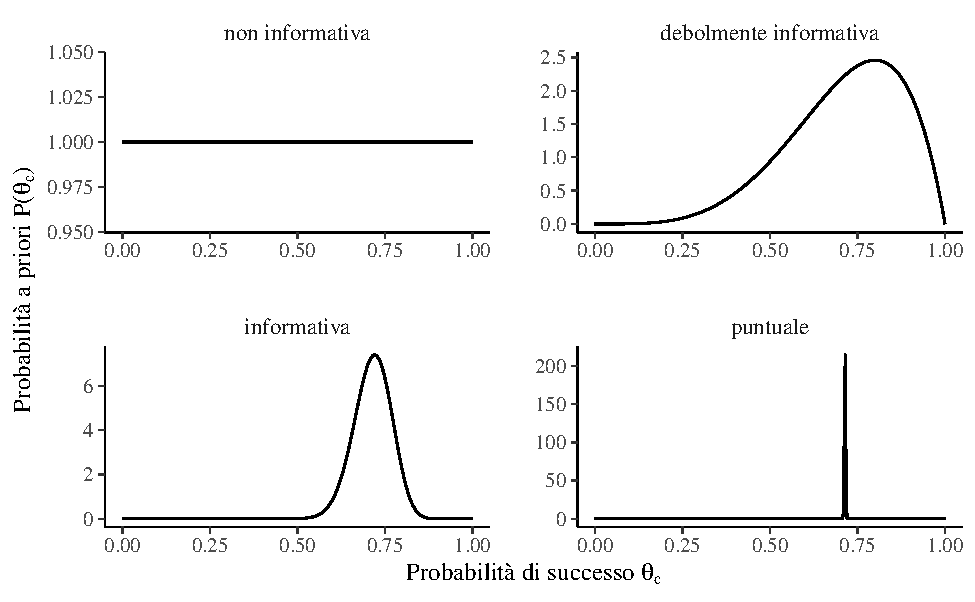
\includegraphics{ds4psy_files/figure-latex/unnamed-chunk-3-1} 

}

\caption{Esempi di distribuzioni a priori per il parametro $\theta_c$ nel Modello Binomiale.}\label{fig:unnamed-chunk-3}
\end{figure}

\hypertarget{selezione-della-distribuzione-a-priori}{%
\subsection{Selezione della distribuzione a priori}\label{selezione-della-distribuzione-a-priori}}

La selezione delle distribuzioni a priori è stata spesso vista come una delle scelte più importanti che un ricercatore fa quando implementa un modello bayesiano in quanto può avere un impatto sostanziale sui risultati finali. La soggettività delle distribuzioni a priori è evidenziata dai critici come un potenziale svantaggio dei metodi bayesiani. A questa critica, \citet{vandeSchoot2021modelling} rispondono dicendo che, al di là della scelta delle distribuzioni a priori, ci sono molti elementi del processo di inferenza statistica che sono soggettivi, ovvero la scelta del modello statistico e le ipotesi sulla distribuzione degli errori. In secondo luogo, \citet{vandeSchoot2021modelling} notano come le distribuzioni a priori svolgono due importanti ruoli statistici: quello della ``regolarizzazione della stima'', ovvero, il processo che porta ad indebolire l'influenza indebita di osservazioni estreme, e quello del miglioramento dell'efficienza della stima, ovvero, la facilitazione dei processi di calcolo numerico di stima della distribuzione a posteriori. L'effetto della distribuzione a priori sulla distribuzione a posteriori verrà discusso in dettaglio nel Capitolo \ref{chapter-balance}.

\hypertarget{unapplicazione-empirica}{%
\subsection{Un'applicazione empirica}\label{unapplicazione-empirica}}

Per introdurre la modelizzazione bayesiana useremo qui i dati riportati da \citet{zetschefuture2019} (si veda l'appendice \ref{appendix:future-exp}). Tali dati corrispondono a 23 ``successi'' in 30 prove e possono dunque essere considerati la manifestazione di una variabile casuale Bernoulliana.

Se non abbiamo alcuna informazione a priori su \(\theta\) (ovvero, la probabilità che l'aspettativa dell'umore futuro del partecipante sia distorta negativamente), potremmo pensare di usare una distribuzione a priori uniforme, ovvero una Beta di parametri \(\alpha=1\) e \(\beta=1\). Una tale scelta, tuttavia, è sconsigliata in quanto è più vantaggioso usare una distribuzione debolmente informativa, come ad esempio \(\mbox{Beta}(2, 2)\), che ha come scopo la regolarizzazione, cioè quello di mantenere le inferenze in un intervallo ragionevole. Qui useremo una \(\mbox{Beta}(2, 10)\).

\[
p(\theta) = \frac{\Gamma(12)}{\Gamma(2)\Gamma(10)}\theta^{2-1} (1-\theta)^{10-1}.
\]

\begin{Shaded}
\begin{Highlighting}[]
\NormalTok{bayesrules}\SpecialCharTok{::}\FunctionTok{plot\_beta}\NormalTok{(}\AttributeTok{alpha =} \DecValTok{2}\NormalTok{, }\AttributeTok{beta =} \DecValTok{10}\NormalTok{, }\AttributeTok{mean =} \ConstantTok{TRUE}\NormalTok{, }\AttributeTok{mode =} \ConstantTok{TRUE}\NormalTok{)}
\end{Highlighting}
\end{Shaded}

\begin{center}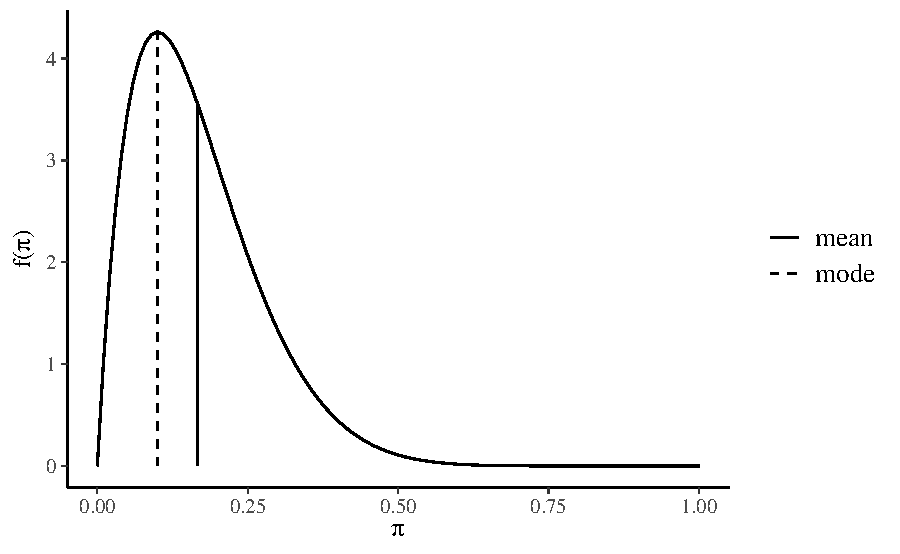
\includegraphics{ds4psy_files/figure-latex/unnamed-chunk-4-1} \end{center}

La \(\mbox{Beta}(2, 10)\) esprime la credenza che \(\theta\) assume valori \(< 0.5\), con il valore più plausibile pari a circa 0.1. Questo è assolutamente implausibile per il caso dell'esempio in discussione: la \(\mbox{Beta}(2, 10)\) verrà usata solo per scopi didattici, ovvero, per esplorare le conseguenze di tale scelta sulla distribuzione a posteriori.

\hypertarget{la-funzione-di-verosimiglianza}{%
\section{La funzione di verosimiglianza}\label{la-funzione-di-verosimiglianza}}

Iniziamo con una definizione.

\begin{definition}
La \emph{funzione di verosimiglianza} \(\mathcal{L}(\theta \mid y) = f(y \mid \theta), \theta \in \Theta,\) è la funzione di massa o di densità di probabilità dei dati \(y\) vista come una funzione del parametro sconosciuto (o dei parametri sconosciuti) \(\theta\).
\end{definition}

Detto in altre parole, le funzioni di verosimiglianza e di (massa o densità di) probabilità sono formalmente identiche, ma è completamente diversa la loro interpretazione. Nel caso della funzione di massa o di densità di probabilità la distribuzione del vettore casuale delle osservazioni campionarie \(y\) dipende dai valori assunti dal parametro (o dai parametri) \(\theta\); nel caso della la funzione di verosimiglianza la credibilità assegnata a ciascun possibile valore \(\theta\) viene determinata avendo acquisita l'informazione campionaria \(y\) che rappresenta l'elemento condizionante. In altri termini, la funzione di verosimiglianza descrive in termini relativi il sostegno empirico che \(\theta \in \Theta\) riceve da \(y\). Infatti, la funzione di verosimiglianza assume forme diverse al variare di \(y\). Possiamo dunque pensare alla funzione di verosimiglianza come alla risposta alla seguente domanda: avendo osservato i dati \(y\), quanto risultano (relativamente) credibili i diversi valori del parametro \(\theta\)? In termini più formali possiamo dire: sulla base dei dati, \(\theta_1 \in \Theta\) risulta più credibile di \(\theta_2 \in \Theta\) quale indice del modello probabilistico generatore dei dati se \(\mathcal{L}(\theta_1) > \mathcal{L}(\theta_1)\).

Notiamo un punto importante: la funzione \(\mathcal{L}(\theta \mid y)\) non è una funzione di densità. Infatti, essa non racchiude un'area unitaria.

\hypertarget{notazione-1}{%
\subsection{Notazione}\label{notazione-1}}

Seguendo una pratica comune, in questa dispensa spesso useremo la notazione \(p(\cdot)\) per rappresentare due quantità differenti, ovvero la funzione di verosimiglianza e la distribuzione a priori. Questo piccolo abuso di notazione riflette il seguente punto di vista: anche se la verosimiglianza non è una funzione di densità di probabilità, noi non vogliamo stressare questo aspetto, ma vogliamo piuttosto pensare alla verosimiglianza e alla distribuzione a priori come a due elementi che sono egualmente necessari per calcolare la distribuzione a posteriori. In altri termini, per così dire, questa notazione assegna lo stesso status epistemologico alle due diverse quantità che si trovano al numeratore della regola di Bayes.

\hypertarget{la-log-verosimiglianza}{%
\subsection{La log-verosimiglianza}\label{la-log-verosimiglianza}}

Dal punto di vista pratico risulta più conveniente utilizzare, al posto della funzione di verosimiglianza, il suo logaritmo naturale, ovvero la funzione di log-verosimiglianza:

\begin{equation}
\ell(\theta) = \log \mathcal{L}(\theta).
\end{equation}

Poiché il logaritmo è una funzione strettamente crescente (usualmente si considera il logaritmo naturale), allora \(\mathcal{L}(\theta)\) e \(\ell(\theta)\) assumono il massimo (o i punti di massimo) in corrispondenza degli stessi valori di \(\theta\) (per un approfondimento, si veda l'Appendice \ref{appendix:max-like}):

\[
\hat{\theta} = \argmax_{\theta \in \Theta} \ell(\theta) = \argmax_{\theta \in \Theta} \mathcal{L}(\theta).
\]

Per le proprietà del logaritmo, si ha

\begin{equation}
\ell(\theta) = \log \left( \prod_{i = 1}^n f(y \mid \theta) \right) = \sum_{i = 1}^n \log f(y \mid \theta).
\end{equation}

Si noti che non è necessario lavorare con i logaritmi, ma è fortemente consigliato. Il motivo è che i valori della verosimiglianza, in cui si moltiplicano valori di probabilità molto piccoli, possono diventare estremamente piccoli -- qualcosa come \(10^{-34}\). In tali circostanze, non è sorprendente che i programmi dei computer mostrino problemi di arrotondamento numerico. Le trasformazioni logaritmiche risolvono questo problema.

\hypertarget{unapplicazione-empirica-1}{%
\subsection{Un'applicazione empirica}\label{unapplicazione-empirica-1}}

Se i dati di \citet{zetschefuture2019} possono essere riassunti da una proporzione allora è sensato adottare un modello probabilistico binomiale quale meccanismo generatore dei dati: \begin{equation}
y  \sim \mbox{Bin}(n, \theta),
\label{eq:binomialmodel}
\end{equation}

laddove \(\theta\) è la probabiltà che una prova Bernoulliana assuma il valore 1 e \(n\) corrisponde al numero di prove Bernoulliane. Questo modello assume che le prove Bernoulliane \(y_i\) che costituiscono il campione \(y\) siano tra loro indipendenti e che ciascuna abbia la stessa probabilità \(\theta \in [0, 1]\) di essere un ``successo'' (valore 1). In altre parole, il modello generatore dei dati avrà una funzione di massa di probabilità

\[
p(y \mid \theta)
\ = \
\mbox{Bin}(y \mid n, \theta).
\]

Nei capitoli precedenti è stato mostrato come, sulla base del modello binomiale, sia possibile assegnare una probabilità a ciascun possibile valore \(y \in \{0, 1, \dots, n\}\) \emph{assumendo noto il valore del parametro} \(\theta\). Ma ora abbiamo il problema inverso, ovvero quello di fare inferenza su \(\theta\) alla luce dei dati campionari \(y\). In altre parole, riteniamo di conoscere il modello probabilistico che ha generato i dati, ma di tale modello non conosciamo i parametri: vogliamo dunque ottenere informazioni su \(\theta\) avendo osservato i dati \(y\).

Per i dati di \citet{zetschefuture2019} la funzione di verosimiglianza corrisponde alla funzione binomiale di parametro \(\theta \in [0, 1]\) sconosciuto. Abbiamo osservato un ``successo'' 23 volte in 30 ``prove'', dunque, \(y = 23\) e \(n = 30\). La funzione di verosimiglianza diventa

\begin{equation}
\mathcal{L}(\theta \mid y) = \frac{(23 + 7)!}{23!7!} \theta^{23} + (1-\theta)^7.
\label{eq:likebino23}
\end{equation}

Per costruire la funzione di verosimiglianza dobbiamo applicare la \eqref{eq:likebino23} tante volte, cambiando ogni volta il valore \(\theta\) ma \emph{tenendo sempre costante il valore dei dati}. Per esempio, se poniamo \(\theta = 0.1\)

\[
\mathcal{L}(\theta \mid y) = \frac{(23 + 7)!}{23!7!} 0.1^{23} + (1-0.1)^7
\]

otteniamo

\begin{Shaded}
\begin{Highlighting}[]
\FunctionTok{dbinom}\NormalTok{(}\DecValTok{23}\NormalTok{, }\DecValTok{30}\NormalTok{, }\FloatTok{0.1}\NormalTok{)}
\CommentTok{\#\textgreater{} [1] 9.737e{-}18}
\end{Highlighting}
\end{Shaded}

Se poniamo \(\theta = 0.2\)

\[
\mathcal{L}(\theta \mid y) = \frac{(23 + 7)!}{23!7!} 0.2^{23} + (1-0.2)^7
\]

otteniamo

\begin{Shaded}
\begin{Highlighting}[]
\FunctionTok{dbinom}\NormalTok{(}\DecValTok{23}\NormalTok{, }\DecValTok{30}\NormalTok{, }\FloatTok{0.2}\NormalTok{)}
\CommentTok{\#\textgreater{} [1] 3.581e{-}11}
\end{Highlighting}
\end{Shaded}

e così via. La figura \ref{fig:likefutexpect} --- costruita utilizzando 100 valori equispaziati \(\theta \in [0, 1]\) --- fornisce una rappresentazione grafica della funzione di verosimiglianza.

\begin{Shaded}
\begin{Highlighting}[]
\NormalTok{n }\OtherTok{\textless{}{-}} \DecValTok{30}
\NormalTok{y }\OtherTok{\textless{}{-}} \DecValTok{23}
\NormalTok{theta }\OtherTok{\textless{}{-}} \FunctionTok{seq}\NormalTok{(}\DecValTok{0}\NormalTok{, }\DecValTok{1}\NormalTok{, }\AttributeTok{length.out =} \DecValTok{100}\NormalTok{)}
\NormalTok{like }\OtherTok{\textless{}{-}} \FunctionTok{choose}\NormalTok{(n, y) }\SpecialCharTok{*}\NormalTok{ theta}\SpecialCharTok{\^{}}\NormalTok{y }\SpecialCharTok{*}\NormalTok{ (}\DecValTok{1} \SpecialCharTok{{-}}\NormalTok{ theta)}\SpecialCharTok{\^{}}\NormalTok{(n }\SpecialCharTok{{-}}\NormalTok{ y)}
\FunctionTok{tibble}\NormalTok{(theta, like) }\SpecialCharTok{\%\textgreater{}\%}
  \FunctionTok{ggplot}\NormalTok{(}\FunctionTok{aes}\NormalTok{(}\AttributeTok{x =}\NormalTok{ theta, }\AttributeTok{y =}\NormalTok{ like)) }\SpecialCharTok{+}
  \FunctionTok{geom\_line}\NormalTok{() }\SpecialCharTok{+}
  \FunctionTok{labs}\NormalTok{(}
    \AttributeTok{y =} \FunctionTok{expression}\NormalTok{(}\FunctionTok{L}\NormalTok{(theta)),}
    \AttributeTok{x =} \FunctionTok{expression}\NormalTok{(}\StringTok{"Valori possibili di"} \SpecialCharTok{\textasciitilde{}}\NormalTok{ theta)}
\NormalTok{  )}
\end{Highlighting}
\end{Shaded}

\begin{figure}[h]

{\centering 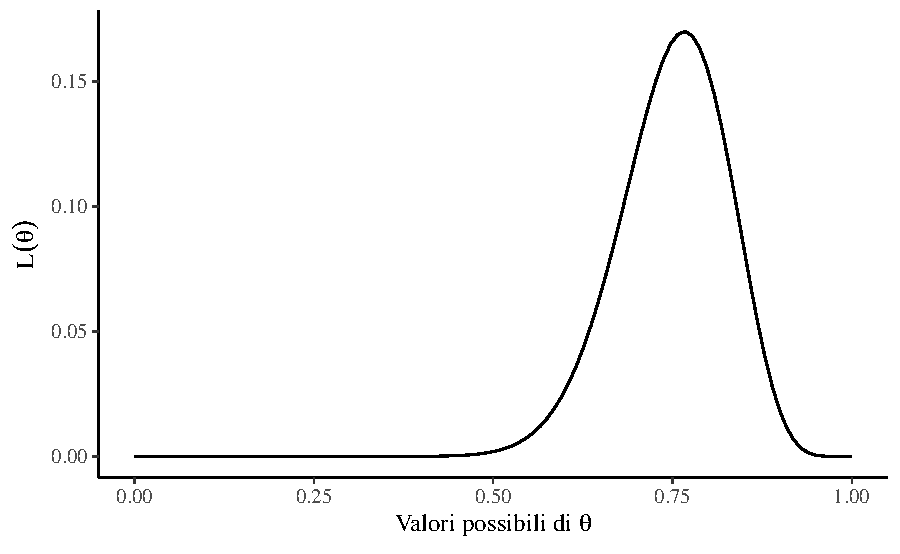
\includegraphics{ds4psy_files/figure-latex/likefutexpect-1} 

}

\caption{Funzione di verosimiglianza nel caso di 23 successi in 30 prove.}\label{fig:likefutexpect}
\end{figure}

Come possiamo interpretare la curva che abbiamo ottenuto? Per alcuni valori \(\theta\) la funzione di verosimiglianza assume valori piccoli; per altri valori \(\theta\) la funzione di verosimiglianza assume valori più grandi. Questi ultimi sono i valori di \(\theta\) più credibili e il valore 23/30 (la moda della funzione di verosimiglianza) è il valore più credibile di tutti.

\hypertarget{sec:const-normaliz-bino23}{%
\section{La verosimiglianza marginale}\label{sec:const-normaliz-bino23}}

Per il calcolo di \(p(\theta \mid y)\) è necessario dividere il prodotto tra la distribuzione a priori e la verosimiglianza per una costante di normalizzazione. Tale costante di normalizzazione, detta \emph{verosimiglianza marginale}, ha lo scopo di fare in modo che \(p(\theta \mid y)\) abbia area unitaria.

Si noti che, nel caso di variabili continue, la verosimiglianza marginale è espressa nei termini di un integrale. Tranne in pochi casi particolari, tale integrale non ha una soluzione analitica. Per questa ragione, l'inferenza bayesiana procede calcolando una approssimazione della distribuzione a posteriori mediante metodi numerici.

\hypertarget{unapplicazione-empirica-2}{%
\subsection{Un'applicazione empirica}\label{unapplicazione-empirica-2}}

Consideriamo nuovamente i dati di \citet{zetschefuture2019}. Supponiamo che nel numeratore bayesiano la verosimiglianza sia moltiplicata per una distribuzione uniforme, ovvero \(\mbox{Beta}(1, 1)\). In tali circostanze, il prodotto si riduce alla funzione di verosimiglianza. Per i dati di \citet{zetschefuture2019}, dunque, la costante di normalizzazione si ottiene marginalizzando la funzione di verosimiglianza \(p(y = 23, n = 30 \mid \theta)\) sopra \(\theta\), ovvero risolvendo l'integrale:

\begin{equation}
p(y = 23, n = 30) = \int_0^1 \binom{30}{23} \theta^{23} (1-\theta)^{7} \,\operatorname {d}\!\theta.
\label{eq:intlikebino23}
\end{equation}

Una soluzione numerica si trova facilmente usando \(\R\):

\begin{Shaded}
\begin{Highlighting}[]
\NormalTok{like\_bin }\OtherTok{\textless{}{-}} \ControlFlowTok{function}\NormalTok{(theta) \{}
  \FunctionTok{choose}\NormalTok{(}\DecValTok{30}\NormalTok{, }\DecValTok{23}\NormalTok{) }\SpecialCharTok{*}\NormalTok{ theta}\SpecialCharTok{\^{}}\DecValTok{23} \SpecialCharTok{*}\NormalTok{ (}\DecValTok{1} \SpecialCharTok{{-}}\NormalTok{ theta)}\SpecialCharTok{\^{}}\DecValTok{7}
\NormalTok{\}}
\FunctionTok{integrate}\NormalTok{(like\_bin, }\AttributeTok{lower =} \DecValTok{0}\NormalTok{, }\AttributeTok{upper =} \DecValTok{1}\NormalTok{)}\SpecialCharTok{$}\NormalTok{value}
\CommentTok{\#\textgreater{} [1] 0.03226}
\end{Highlighting}
\end{Shaded}

La derivazione analitica è fornita nell'Appendice \ref{appendix:const-norm-bino23}.

\hypertarget{distribuzione-a-posteriori}{%
\section{Distribuzione a posteriori}\label{distribuzione-a-posteriori}}

La distribuzione a postreriori si trova applicando il teorema di Bayes:

\[
\text{probabilità a posteriori} = \frac{\text{probabilità a priori} \cdot \text{verosimiglianza}}{\text{costante di normalizzazione}}
\]

Una volta trovata la distribuzione a posteriori, possiamo usarla per derivare altre quantità di interesse. Questo viene generalmente ottenuto calcolando il valore atteso:

\[
J = \int f(\theta) p(\theta \mid y) \,\operatorname {d}\!y
\]

Se \(f(\cdot)\) è la funzione identità, ad esempio, \(J\) risulta essere la media di \(\theta\):

\[
\bar{\theta} = \int_{\Theta} \theta p(\theta \mid y) \,\operatorname {d}\!\theta .
\]

Ripeto qui quanto detto sopra: le quantità di interesse della statistica bayesiana(costante di normalizzazione, valore atteso della distribuzione a posteriori, ecc.) contengono integrali che risultano, nella maggior parte dei casi, impossibili da risolvere analiticamente. Per questo motivo, si ricorre a metodi di stima numerici, in particolare a quei metodi Monte Carlo basati sulle proprietà delle catene di Markov (MCMC). Questo argomento verrà discusso nel Capitolo \ref{ch:metropolis}.

\hypertarget{distribuzione-predittiva-a-priori}{%
\section{Distribuzione predittiva a priori}\label{distribuzione-predittiva-a-priori}}

La distribuzione a posteriori è l'oggetto centrale nella statistica bayesiana, ma non è l'unico. Oltre a fare inferenze sui valori dei parametri, potremmo voler fare inferenze sui dati. Questo può essere fatto calcolando la \emph{distribuzione predittiva a priori}:

\begin{equation}
p(y^*) = \int_\Theta p(y^* \mid \theta) p(\theta) \,\operatorname {d}\!\theta .
\label{eq:prior-pred-distr}
\end{equation}

La \eqref{eq:prior-pred-distr} descrive la distribuzione prevista dei dati in base al modello (che include la distribuzione a priori e la verosimiglianza), ovvero descrive i dati \(y^*\) che ci aspettiamo di osservare, dato il modello, prima di avere osservato i dati del campione.

È possibile utilizzare campioni dalla distribuzione predittiva a priori per valutare e calibrare i modelli utilizzando le nostre conoscenze dominio-specifiche. Ad esempio, ci possiamo chiedere: ``È sensato che un modello dell'altezza umana preveda che un essere umano sia alto -1.5 metri?''. Già prima di misurare una singola persona, possiamo renderci conto dell'assurdità di questa domanda. Se la distribuzione prevista dei dati consente domande di questo tipo (ovvero, prevede di osservare dati che risultano insensati alla luce delle nostre conoscenze dominio-specifiche), è chiaro che il modello deve essere riformulato.

\hypertarget{distribuzione-predittiva-a-posteriori}{%
\section{Distribuzione predittiva a posteriori}\label{distribuzione-predittiva-a-posteriori}}

Un'altra quantità utile da calcolare è la distribuzione predittiva a posteriori:

\begin{equation}
p(\tilde{y} \mid y) = \int_\Theta p(\tilde{y} \mid \theta) p(\theta \mid y) \,\operatorname {d}\!\theta .
\label{eq:post-pred-distr}
\end{equation}

Questa è la distribuzione dei dati attesi futuri \(\tilde{y}\) alla luce della distribuzione a posteriori \(p(\theta \mid y)\), che a sua volta è una conseguenza del modello adottato (distribuzione a priori e verosimiglianza) e dei dati osservati. In altre parole, questi sono i dati che il modello si aspetta dopo aver osservato i dati de campione. Dalla \eqref{eq:post-pred-distr} possiamo vedere che le previsioni sui dati attesi futuri sono calcolate integrando (o marginalizzando) sulla distribuzione a posteriori dei parametri. Di conseguenza, le previsioni calcolate in questo modo incorporano l'incertezza relativa alla stima dei parametri del modello.

\hypertarget{commenti-e-considerazioni-finali}{%
\section*{Commenti e considerazioni finali}\label{commenti-e-considerazioni-finali}}


Questo Capitolo ha brevemente passato in rassegna i concetti di base dell'inferenza statistica bayesiana. In base all'approccio bayesiano, invece di dire che il parametro di interesse di un modello statistico ha un valore vero ma sconosciuto, diciamo che, prima di eseguire l'esperimento, è possibile assegnare una distribuzione di probabilità, che chiamano stato di credenza, a quello che è il vero valore del parametro. Questa distribuzione a priori può essere nota (per esempio, sappiamo che la distribuzione dei punteggi del QI è normale con media 100 e deviazione standard 15) o può essere del tutto arbitraria. L'inferenza bayesiana procede poi nel modo seguente: si raccolgono alcuni dati e si calcola la probabilità dei possibili valori del parametro alla luce dei dati osservati e delle credenze a priori. Questa nuova distribuzione di probabilità è chiamata ``distribuzione a posteriori'' e riassume l'incertezza dell'inferenza.

\hypertarget{ch-subj-think-prop}{%
\chapter{Pensare ad una proporzione in termini soggettivi}\label{ch-subj-think-prop}}

Obiettivo di questo Capitolo è introdurre l'inferenza bayesiana considerando il caso della verosimiglianza binomiale. Esamineremo prima il caso di una distribuzione a priori è discreta; poi considereremo una distribuzione a priori continua. Il materiale che presento qui è un semplice riassunto del capitolo 7 del testo di \citet{albert2019probability}.

\hypertarget{ch-prior-discr-binom}{%
\section{Inferenza bayesiana con una distribuzione a priori discreta}\label{ch-prior-discr-binom}}

Nei problemi tradizionali di teoria delle probabilità ci sono molti esempi che riguardano l'estrazione di palline colorate da un'urna. In questi esempi, ci viene fornito il numero di palline di vari colori presenti nell'urna e ci viene chiesto di calcolare le probabilità di vari eventi. Ad esempio, in un'urna ci sono 40 palline bianche e 20 rosse. Se estrai due palline a caso, qual è la probabilità che entrambe siano bianche?

L'approccio bayesiano considera uno scenario diverso, ovvero quello in cui non conosciamo le proporzioni delle palline colorate presenti nell'urna. Cioè, nell'esempio precedente, sappiamo solo che nell'urna ci sono due tipi di palline colorate, ma non sappiamo che 40 sono bianche (proporzione di bianco = \(2/3\)) e 20 sono rosse (proporzione di rosso = \(1/3\)). Ci poniamo la seguente domanda: è possibile inferire le proporzioni di palline nell'urna estraendo un campione di palline dall'urna e osservando i colori delle palline nel campione? Espresso in questo modo, questo diventa un problema di inferenza statistica, perché stiamo cercando di inferire la proporzione \(\pi\) della popolazione sulla base di un campione casuale. Per continuare con l'esempio precedente, quello che vogliamo fare è inferire \(\pi\), la proporzione di palline rosse nell'urna, in base al numero di palline rosse e bianche che osserviamo nel campione.

Le proporzioni assomigliano alle probabilità. Ricordiamo che sono state proposte tre diverse interpretazioni del concetto di una probabilità.

\begin{itemize}
\tightlist
\item
  Il punto di vista classico: è necessario enumerare tutti gli eventi elementari dello spazio campionario in cui ogni risultato è ugualmente probabile.
\item
  Il punto di vista frequentista: è necessario ripetere l'esperimento esperimento casuale (cioè l'estrazione del campione) molte volte in condizioni identiche.
\item
  La visione soggettiva: è necessario esprimere la propria opinione sulla probabilità di un evento unico e irripetibile.
\end{itemize}

La visione classica non sembra potere funzionare qui, perché sappiamo solo che ci sono due tipi di palline colorate e il numero totale di palline è 60. Anche se estraiamo un campione di 10 palline, possiamo solo osservare la proporzione di palline rosse palline nel campione. Non c'è modo per stabilire quali sono le proprietà dello spazio campionario in cui ogni risultato è ugualmente probabile.

La visione frequentista potrebbe funzionare nel caso presente. Possiamo considerare il processo del campionamento (cioè l'estrazione di un campione casuale di 10 palline dall'urna) come un esperimento casuale che produce una proporzione campionaria \(p\). Potremmo quindi pensare di ripetere l'esperimento molte volte nelle stesse condizioni, ottenere molte proporzioni campionarie \(p\) e riassumere poi in qualche modo questa distribuzione di statistiche campionarie. Ripetendo l'esperimento casuale tante volte è possibile ottenere una stima abbastanza accurata della proporzione \(\pi\) di palline rosse nell'urna. Questo processo è fattibile, ma è però noioso, dispendioso in termini di tempo e soggetto ad errori.

La visione soggettivista concepisce invece la probabilità sconosciuta \(\pi\) come un'opinione soggettiva di cui possiamo essere più o meno sicuri. Abbiamo visto in precedenza come questa opinione soggettiva dipenda da due tipi di evidenze: le nostre credenze iniziali e le nuove informazioni fornite dai dati che abbiamo osservato. Vedremo in questo capitolo come sia possibile combinare le credenze iniziali rispetto al possibile valore \(\pi\) con le evidenza fornite dai dati per giungere ad una credenza a posteriori su \(\pi\). In particolare, vedremo come si possa pensare in termini soggetti a delle quantità sconosciute (in questo caso, \(\pi\)) usando le distribuzioni di probabilità.

Sappiamo che, essendo una proporzione, \(\pi\) può assumere valori compresi tra 0 e 1. Potremmo pensare che \(\pi\) sia uguale, ad esempio, a 0.5. Ciò significa assegnare all'evento \(\pi = 1\) la probabilità 1 -- in altri termini, significa dire che siamo assolutamente certi che la quantità sconosciuta \(\pi\) ha il valore di 0.5. Questa posizione, però, è troppo estrema: non possiamo essere assolutamente certi che una quantità sconosciuta abbia uno specifico valore; altrimenti non sarebbe una quantità sconosciuta. Invece, sembra più sensato pensare che \(\pi\) può, in linea di principio, assumere valori diversi e, a questi valori, vengono attribuiti diversi livelli di certezza soggettiva. Consideriamo, ad esempio, 10 possibili valori per \(\pi\):

\begin{Shaded}
\begin{Highlighting}[]
\NormalTok{pi }\OtherTok{\textless{}{-}} \FunctionTok{seq}\NormalTok{(}\FloatTok{0.1}\NormalTok{, }\DecValTok{1}\NormalTok{, }\AttributeTok{length.out =} \DecValTok{10}\NormalTok{)}
\NormalTok{pi}
\CommentTok{\#\textgreater{}  [1] 0.1 0.2 0.3 0.4 0.5 0.6 0.7 0.8 0.9 1.0}
\end{Highlighting}
\end{Shaded}

Se non abbiamo alcun motivo di pensare diversamente, potremmo pensare di assegnare a ciascuno di questi valori lo stesso livello di plausibilità:

\begin{Shaded}
\begin{Highlighting}[]
\NormalTok{p1 }\OtherTok{\textless{}{-}} \FunctionTok{rep}\NormalTok{(}\FloatTok{0.1}\NormalTok{, }\DecValTok{10}\NormalTok{)}
\NormalTok{p1}
\CommentTok{\#\textgreater{}  [1] 0.1 0.1 0.1 0.1 0.1 0.1 0.1 0.1 0.1 0.1}
\end{Highlighting}
\end{Shaded}

\begin{Shaded}
\begin{Highlighting}[]
\FunctionTok{tibble}\NormalTok{(pi, p1) }\SpecialCharTok{\%\textgreater{}\%}
  \FunctionTok{ggplot}\NormalTok{(}\FunctionTok{aes}\NormalTok{(pi, p1)) }\SpecialCharTok{+}
  \FunctionTok{geom\_segment}\NormalTok{(}
    \FunctionTok{aes}\NormalTok{(}\AttributeTok{xend =}\NormalTok{ pi, }\AttributeTok{yend =} \DecValTok{0}\NormalTok{),}
    \AttributeTok{size =} \DecValTok{10}\NormalTok{, }\AttributeTok{lineend =} \StringTok{"butt"}
\NormalTok{  )}
\end{Highlighting}
\end{Shaded}

\begin{center}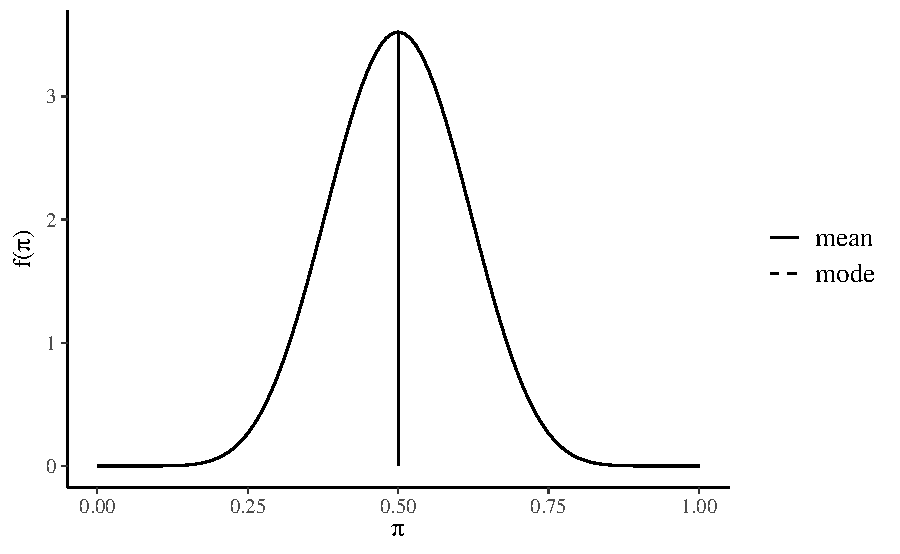
\includegraphics{ds4psy_files/figure-latex/unnamed-chunk-11-1} \end{center}

Oppure, per qualche ragione, potremmo pensare che i valori centrali della distribuzione di \(\pi\) siamo più plausibili dei valori estremi. Tale opinione soggettiva potrebbe corrispondere alla seguente distribuzione di massa di probabilità:

\begin{Shaded}
\begin{Highlighting}[]
\NormalTok{p2 }\OtherTok{\textless{}{-}} \FunctionTok{c}\NormalTok{(}
  \FloatTok{0.05}\NormalTok{, }\FloatTok{0.05}\NormalTok{, }\FloatTok{0.05}\NormalTok{, }\FloatTok{0.175}\NormalTok{, }\FloatTok{0.175}\NormalTok{, }\FloatTok{0.175}\NormalTok{, }\FloatTok{0.175}\NormalTok{, }\FloatTok{0.05}\NormalTok{, }\FloatTok{0.05}\NormalTok{, }\FloatTok{0.05}
\NormalTok{)}
\NormalTok{p2}
\CommentTok{\#\textgreater{}  [1] 0.050 0.050 0.050 0.175 0.175 0.175 0.175 0.050}
\CommentTok{\#\textgreater{}  [9] 0.050 0.050}
\end{Highlighting}
\end{Shaded}

\begin{Shaded}
\begin{Highlighting}[]
\FunctionTok{tibble}\NormalTok{(pi, p2) }\SpecialCharTok{\%\textgreater{}\%}
  \FunctionTok{ggplot}\NormalTok{(}\FunctionTok{aes}\NormalTok{(pi, p2)) }\SpecialCharTok{+}
  \FunctionTok{geom\_segment}\NormalTok{(}
    \FunctionTok{aes}\NormalTok{(}\AttributeTok{xend =}\NormalTok{ pi, }\AttributeTok{yend =} \DecValTok{0}\NormalTok{),}
    \AttributeTok{size =} \DecValTok{10}\NormalTok{, }\AttributeTok{lineend =} \StringTok{"butt"}
\NormalTok{  )}
\end{Highlighting}
\end{Shaded}

\begin{center}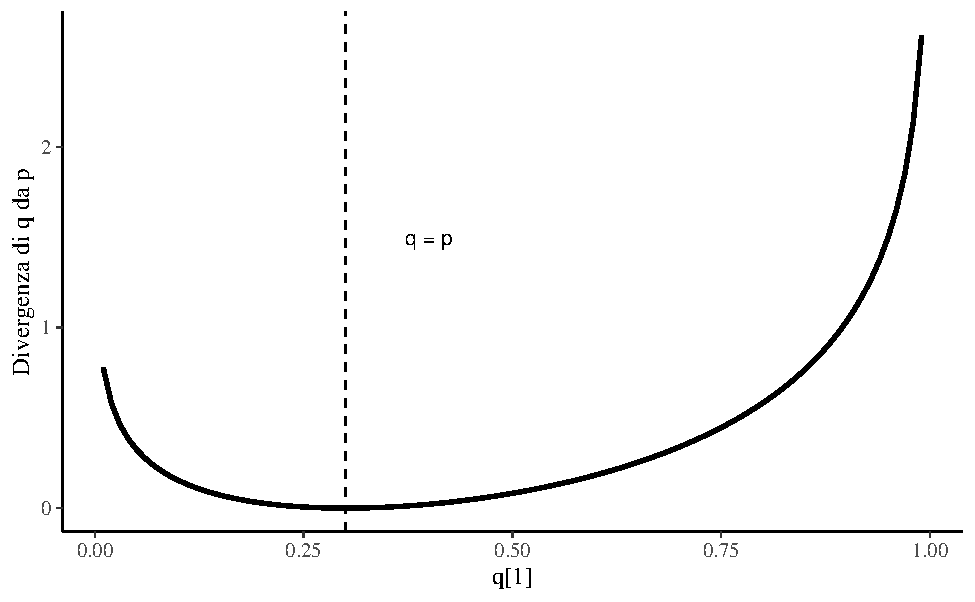
\includegraphics{ds4psy_files/figure-latex/unnamed-chunk-13-1} \end{center}

La prima distribuzione di probabilità è chiamata distribuzione discreta uniforme perché attribuisce la stessa probabilità (ovvero, 1/10) ad ogni elemento dell'insieme discreto su cui è definita (ovvero, \(0.1, 0.2, \dots, 1.0\)). Anche la seconda distribuzione è discreta, ma non è uniforme: viene ritenuto più plausibile che \(\pi\) assuma un valore nell'insieme \(\{0.4, 0.5, 0.6, 0.7\}\) piuttosto che nell'insieme \(\{0.1, 0.2, 0.3, 0.8, 0.9, 1.0\}\).

Le credenze relative alla plausibilità dei possibili valori che \(\pi\) possono assumere forme diverse e corrispondono a quella che viene chiamata la \emph{distribuzione a priori}, ovvero descrivono le credenze che possediamo relativamente alla quantità sconosciuta di interesse.

La procedura di inferenza bayesiana non fa altro che ``aggiornare'' tali credenze a priori utilizzando le informazioni fornite da un campione di dati. Usando il teorema di Bayes, le informazioni dei dati vengono combinate con le nostre precedenti credenze relative alla quantità sconosciuta \(\pi\) per giungere ad una credenza detta ``a posteriori''.

Supponendo che i dati corrispondano all'osservazione di 12 palline rosse in 20 estrazioni con rimessa dall'urna, usiamo ora la seconda delle distribuzioni a priori descritte in precedenza per ottenere la distribuzione a posteriori. Il teorema di Bayes specifica la distribuzione a posteriori come il prodotto della verosimiglianza e la distribuzione a priori, diviso per una costante di normalizzazione:

\[
p(\theta \mid y) = \frac{p(y \mid \theta)p(\theta)}{p(y)}.
\]

Per definire la funzione di verosimiglianza, \(p(y \mid \theta)\), è necessario pensare a come abbiamo ottenuto i dati. Abbiamo estratto 20 palline dall'una, con rimessa. Dunque, se l'estrazione è stata casuale con reinserimento, allora i dati (12 successi in 20 prove) possono essere intesi come il risultato di un esperimento casuale binomiale. Usando \(\textsf{R}\), la funzione di verosimiglianza è dunque data da:

\begin{Shaded}
\begin{Highlighting}[]
\NormalTok{like }\OtherTok{\textless{}{-}} \FunctionTok{dbinom}\NormalTok{(}\DecValTok{12}\NormalTok{, }\DecValTok{20}\NormalTok{, pi)}
\NormalTok{like}
\CommentTok{\#\textgreater{}  [1] 5.423e{-}08 8.657e{-}05 3.859e{-}03 3.550e{-}02 1.201e{-}01}
\CommentTok{\#\textgreater{}  [6] 1.797e{-}01 1.144e{-}01 2.216e{-}02 3.558e{-}04 0.000e+00}
\end{Highlighting}
\end{Shaded}

\begin{Shaded}
\begin{Highlighting}[]
\FunctionTok{tibble}\NormalTok{(pi, like) }\SpecialCharTok{\%\textgreater{}\%}
  \FunctionTok{ggplot}\NormalTok{(}\FunctionTok{aes}\NormalTok{(pi, like)) }\SpecialCharTok{+}
  \FunctionTok{geom\_segment}\NormalTok{(}
    \FunctionTok{aes}\NormalTok{(}\AttributeTok{xend =}\NormalTok{ pi, }\AttributeTok{yend =} \DecValTok{0}\NormalTok{),}
    \AttributeTok{size =} \DecValTok{10}\NormalTok{, }\AttributeTok{lineend =} \StringTok{"butt"}
\NormalTok{  )}
\end{Highlighting}
\end{Shaded}

\begin{center}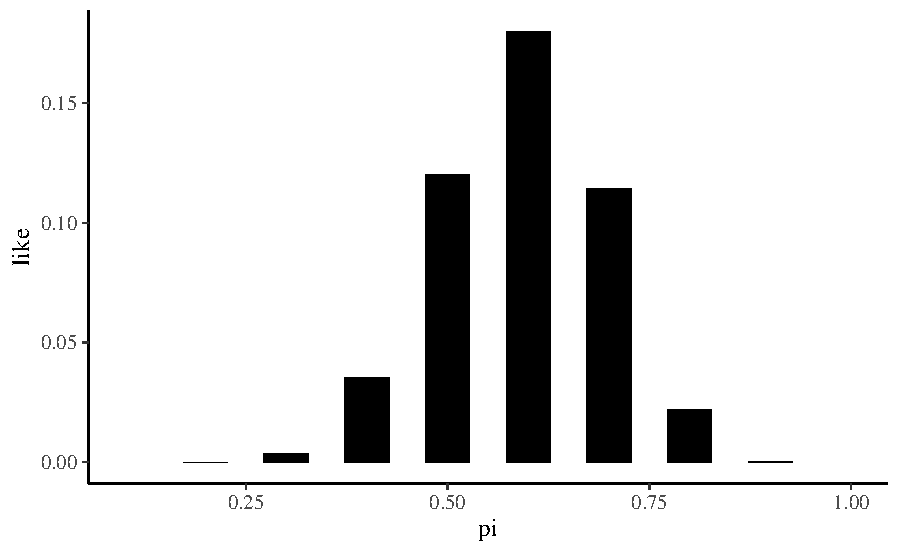
\includegraphics{ds4psy_files/figure-latex/unnamed-chunk-15-1} \end{center}

Per calcolare la distribuzione a posteriori dobbiamo dunque fare il prodotto (elemento per elemento) del vettore che contiene i valori della distribuzione a priori per il vettore che contiene i valori di verosimiglianza. Tale prodotto andrà poi diviso per una costante di normalizzazione, \(p(y)\).

Per la legge della probabilità totale, il denominatore corrisponde alla probabilità marginale dei dati \(y\) ed è uguale alla somma dei prodotti tra la distribuzione a priori e la verosimiglianza calcolata in corrispondenza di ciascun valore possibile di \(\pi\).

Nel nostro caso discreto, la probabilità marginale dei dati ci calcola utilizzando la distribuzione a priori

\begin{Shaded}
\begin{Highlighting}[]
\NormalTok{p2}
\CommentTok{\#\textgreater{}  [1] 0.050 0.050 0.050 0.175 0.175 0.175 0.175 0.050}
\CommentTok{\#\textgreater{}  [9] 0.050 0.050}
\end{Highlighting}
\end{Shaded}

e la verosimiglianza

\begin{Shaded}
\begin{Highlighting}[]
\NormalTok{like}
\CommentTok{\#\textgreater{}  [1] 5.423e{-}08 8.657e{-}05 3.859e{-}03 3.550e{-}02 1.201e{-}01}
\CommentTok{\#\textgreater{}  [6] 1.797e{-}01 1.144e{-}01 2.216e{-}02 3.558e{-}04 0.000e+00}
\end{Highlighting}
\end{Shaded}

Dopo avere fatto il prodotto

\begin{Shaded}
\begin{Highlighting}[]
\NormalTok{p2 }\SpecialCharTok{*}\NormalTok{ like}
\CommentTok{\#\textgreater{}  [1] 2.711e{-}09 4.328e{-}06 1.930e{-}04 6.212e{-}03 2.102e{-}02}
\CommentTok{\#\textgreater{}  [6] 3.145e{-}02 2.002e{-}02 1.108e{-}03 1.779e{-}05 0.000e+00}
\end{Highlighting}
\end{Shaded}

dobbiamo sommare:

\begin{Shaded}
\begin{Highlighting}[]
\FunctionTok{sum}\NormalTok{(p2 }\SpecialCharTok{*}\NormalTok{ like)}
\CommentTok{\#\textgreater{} [1] 0.08003}
\end{Highlighting}
\end{Shaded}

Una volta calcolata la verosimiglianza marginale dei dati, possiamo trovare la distribuzione a posteriori di \(\pi\):

\begin{Shaded}
\begin{Highlighting}[]
\NormalTok{post }\OtherTok{\textless{}{-}}\NormalTok{ (p2 }\SpecialCharTok{*}\NormalTok{ like) }\SpecialCharTok{/} \FunctionTok{sum}\NormalTok{(p2 }\SpecialCharTok{*}\NormalTok{ like)}
\NormalTok{post}
\CommentTok{\#\textgreater{}  [1] 3.388e{-}08 5.409e{-}05 2.411e{-}03 7.762e{-}02 2.627e{-}01}
\CommentTok{\#\textgreater{}  [6] 3.930e{-}01 2.502e{-}01 1.385e{-}02 2.223e{-}04 0.000e+00}
\end{Highlighting}
\end{Shaded}

\begin{Shaded}
\begin{Highlighting}[]
\FunctionTok{tibble}\NormalTok{(pi, post) }\SpecialCharTok{\%\textgreater{}\%}
  \FunctionTok{ggplot}\NormalTok{(}\FunctionTok{aes}\NormalTok{(pi, post)) }\SpecialCharTok{+}
  \FunctionTok{geom\_segment}\NormalTok{(}
    \FunctionTok{aes}\NormalTok{(}\AttributeTok{xend =}\NormalTok{ pi, }\AttributeTok{yend =} \DecValTok{0}\NormalTok{),}
    \AttributeTok{size =} \DecValTok{10}\NormalTok{, }\AttributeTok{lineend =} \StringTok{"butt"}
\NormalTok{  )}
\end{Highlighting}
\end{Shaded}

\begin{center}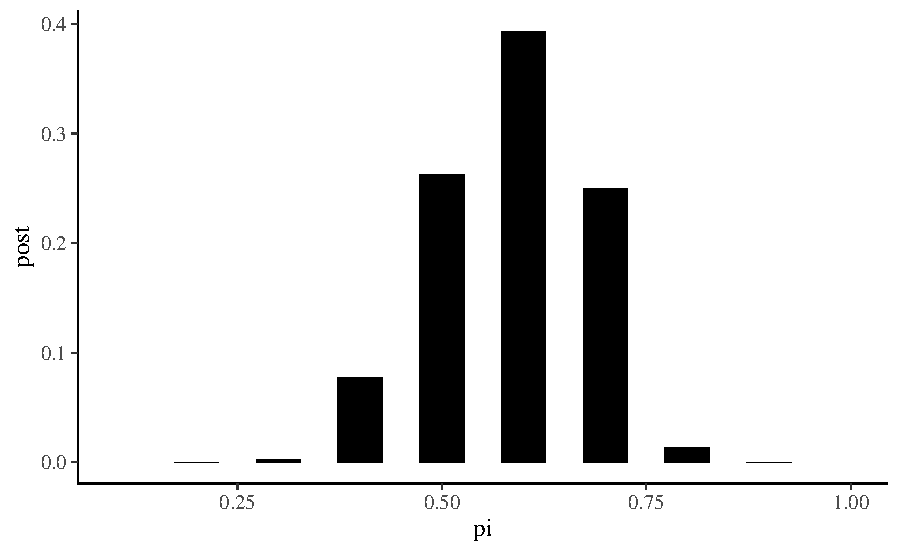
\includegraphics{ds4psy_files/figure-latex/unnamed-chunk-21-1} \end{center}

Conoscendo la distribuzione a posteriori di \(\pi\) diventa possibile calcolare altre quantità di interesse. Per esempio, la moda a posteriori di \(\pi\) si ricava direttamente dal grafico precedente, e corrisponde a 0.6. La media a posteriori è data da:

\begin{Shaded}
\begin{Highlighting}[]
\FunctionTok{sum}\NormalTok{(pi }\SpecialCharTok{*}\NormalTok{ post)}
\CommentTok{\#\textgreater{} [1] 0.5853}
\end{Highlighting}
\end{Shaded}

La varianza della distribuzione a posteriori è

\begin{Shaded}
\begin{Highlighting}[]
\FunctionTok{sum}\NormalTok{(pi}\SpecialCharTok{\^{}}\DecValTok{2} \SpecialCharTok{*}\NormalTok{ post) }\SpecialCharTok{{-}}\NormalTok{ (}\FunctionTok{sum}\NormalTok{(pi }\SpecialCharTok{*}\NormalTok{ post))}\SpecialCharTok{\^{}}\DecValTok{2}
\CommentTok{\#\textgreater{} [1] 0.008817}
\end{Highlighting}
\end{Shaded}

Il calcolo della distribuzione a posteriori, nel caso di una distribuzione a priori discreta, è implementata nella funzione \texttt{bayesian\_crank()} del pacchetto \texttt{ProbBayes}. Dato che \texttt{ProbBayes} non è su CRAN, può essere installato nel modo seguente:

\begin{Shaded}
\begin{Highlighting}[]
\FunctionTok{library}\NormalTok{(}\StringTok{"devtools"}\NormalTok{)}
\FunctionTok{install\_github}\NormalTok{(}\StringTok{"bayesball/ProbBayes"}\NormalTok{)}
\end{Highlighting}
\end{Shaded}

Una volta installato, il pacchetto può essere caricato come facciamo normalmente:

\begin{Shaded}
\begin{Highlighting}[]
\FunctionTok{library}\NormalTok{(}\StringTok{"ProbBayes"}\NormalTok{)}
\end{Highlighting}
\end{Shaded}

Per usare \texttt{bayesian\_crank()} procediamo come indicato di seguito:

\begin{Shaded}
\begin{Highlighting}[]
\NormalTok{df }\OtherTok{\textless{}{-}} \FunctionTok{tibble}\NormalTok{(}\AttributeTok{p =}\NormalTok{ pi, }\AttributeTok{Prior =}\NormalTok{ p2)}
\NormalTok{y }\OtherTok{\textless{}{-}} \DecValTok{12}
\NormalTok{n }\OtherTok{\textless{}{-}} \DecValTok{20}
\NormalTok{df}\SpecialCharTok{$}\NormalTok{Likelihood }\OtherTok{\textless{}{-}} \FunctionTok{dbinom}\NormalTok{(y, }\AttributeTok{prob =}\NormalTok{ df}\SpecialCharTok{$}\NormalTok{p, }\AttributeTok{size =}\NormalTok{ n)}
\NormalTok{df }\OtherTok{\textless{}{-}} \FunctionTok{bayesian\_crank}\NormalTok{(df)}
\NormalTok{df}
\CommentTok{\#\textgreater{} \# A tibble: 10 x 5}
\CommentTok{\#\textgreater{}       p Prior   Likelihood       Product    Posterior}
\CommentTok{\#\textgreater{}   \textless{}dbl\textgreater{} \textless{}dbl\textgreater{}        \textless{}dbl\textgreater{}         \textless{}dbl\textgreater{}        \textless{}dbl\textgreater{}}
\CommentTok{\#\textgreater{} 1   0.1 0.05  0.0000000542 0.00000000271 0.0000000339}
\CommentTok{\#\textgreater{} 2   0.2 0.05  0.0000866    0.00000433    0.0000541   }
\CommentTok{\#\textgreater{} 3   0.3 0.05  0.00386      0.000193      0.00241     }
\CommentTok{\#\textgreater{} 4   0.4 0.175 0.0355       0.00621       0.0776      }
\CommentTok{\#\textgreater{} 5   0.5 0.175 0.120        0.0210        0.263       }
\CommentTok{\#\textgreater{} 6   0.6 0.175 0.180        0.0314        0.393       }
\CommentTok{\#\textgreater{} 7   0.7 0.175 0.114        0.0200        0.250       }
\CommentTok{\#\textgreater{} 8   0.8 0.05  0.0222       0.00111       0.0138      }
\CommentTok{\#\textgreater{} \# ... with 2 more rows}
\end{Highlighting}
\end{Shaded}

Verifichiamo il risultato trovato calcolando, ad esempio, la media a posteriori (come abbiamo fatto sopra):

\begin{Shaded}
\begin{Highlighting}[]
\FunctionTok{sum}\NormalTok{(pi }\SpecialCharTok{*}\NormalTok{ df}\SpecialCharTok{$}\NormalTok{Posterior)}
\CommentTok{\#\textgreater{} [1] 0.5853}
\end{Highlighting}
\end{Shaded}

In questo modo possiamo dunque trovare la distribuzione a posteriori per \(\pi\), nel caso di qualunque distribuzione a priori discreta.

\hypertarget{ch-prior-cont-binom}{%
\section{Inferenza bayesiana con una distribuzione a priori continua}\label{ch-prior-cont-binom}}

Il caso di una distribuzione a priori discreta è stato discusso solo per scopi didattici. In generale, però, l'uso di una distribuzione a priori discreta non è una buona scelta per rappresentare le nostre credenze a priori sul parametro sconosciuto. Infatti, per definizione, una distribuzione a priori discreta può rappresentare solo alcuni dei possibili valori del parametro -- nel caso dell'esempio precedente, non abbiamo considerato il valore 0.55, per esempio. Sembra molto più sensato descrivere le nostre credenze a priori sul parametro utilizzando una distribuzione continua.

Cerchiamo una funzione di densità con supporto in \([0, 1]\). Il candidato naturale è ovviamente fornito dalla funzione Beta (si veda il Capitolo \ref{distr-rv-cont}). Come per le altre funzioni di densità, abbiamo a disposizione quattro funzioni \(\textsf{r}\) che ci consentono di manipolare facilmente questa densità.

\begin{itemize}
\tightlist
\item
  Ad esempio, possiao valutare la funzione di densità \(\mbox{Beta}(1, 1)\) in corrispondenza dei valori \(p = 0.5\) e \(p = 0.8\), che dovrebbe essere entrambi uguali a 1, e in corrispondenza di \(p = 1.2\), che dovrebbe essere ugualea 0 poiché questo valore è al di fuori dell'intervallo \([ 0, 1]\).
\end{itemize}

\begin{Shaded}
\begin{Highlighting}[]
\FunctionTok{dbeta}\NormalTok{(}\FunctionTok{c}\NormalTok{(}\FloatTok{0.5}\NormalTok{, }\FloatTok{0.8}\NormalTok{, }\FloatTok{1.2}\NormalTok{), }\DecValTok{1}\NormalTok{, }\DecValTok{1}\NormalTok{)}
\CommentTok{\#\textgreater{} [1] 1 1 0}
\end{Highlighting}
\end{Shaded}

Oppure possiamo valutare la funzione distribuzione \(\mbox{Beta}(1, 1)\) in corrispondenza dei punti 0.5 e 0.8:

\begin{Shaded}
\begin{Highlighting}[]
\FunctionTok{pbeta}\NormalTok{(}\FunctionTok{c}\NormalTok{(}\FloatTok{0.5}\NormalTok{, }\FloatTok{0.8}\NormalTok{), }\DecValTok{1}\NormalTok{, }\DecValTok{1}\NormalTok{)}
\CommentTok{\#\textgreater{} [1] 0.5 0.8}
\end{Highlighting}
\end{Shaded}

Oppure possiamo calcolare la probabilità \(P(0.5 < p < 0.8)\)

\begin{Shaded}
\begin{Highlighting}[]
\FunctionTok{pbeta}\NormalTok{(}\FloatTok{0.8}\NormalTok{, }\DecValTok{1}\NormalTok{, }\DecValTok{1}\NormalTok{) }\SpecialCharTok{{-}} \FunctionTok{pbeta}\NormalTok{(}\FloatTok{0.5}\NormalTok{, }\DecValTok{1}\NormalTok{, }\DecValTok{1}\NormalTok{)}
\CommentTok{\#\textgreater{} [1] 0.3}
\end{Highlighting}
\end{Shaded}

Possiamo trovare i quntili della distribuzione \(\mbox{Beta}(1, 1)\) di ordine 0.5 e 0.8:

\begin{Shaded}
\begin{Highlighting}[]
\FunctionTok{qbeta}\NormalTok{(}\FunctionTok{c}\NormalTok{(}\FloatTok{0.5}\NormalTok{, }\FloatTok{0.8}\NormalTok{), }\DecValTok{1}\NormalTok{, }\DecValTok{1}\NormalTok{)}
\CommentTok{\#\textgreater{} [1] 0.5 0.8}
\end{Highlighting}
\end{Shaded}

Infine, è possibile simulare dei valori casuali dalla distribuzione \(\mbox{Beta}(1, 1)\). Se vogliamo 5 valori, scriviamo:

\begin{Shaded}
\begin{Highlighting}[]
\FunctionTok{rbeta}\NormalTok{(}\DecValTok{5}\NormalTok{, }\DecValTok{1}\NormalTok{, }\DecValTok{1}\NormalTok{)}
\CommentTok{\#\textgreater{} [1] 0.2523 0.5493 0.2174 0.4064 0.2129}
\end{Highlighting}
\end{Shaded}

Se vogliamo 5 valori da una \(\mbox{Beta}(2, 10)\), scriviamo:

\begin{Shaded}
\begin{Highlighting}[]
\FunctionTok{rbeta}\NormalTok{(}\DecValTok{5}\NormalTok{, }\DecValTok{2}\NormalTok{, }\DecValTok{10}\NormalTok{)}
\CommentTok{\#\textgreater{} [1] 0.17365 0.21333 0.24431 0.15818 0.04897}
\end{Highlighting}
\end{Shaded}

Il pacchetto \texttt{ProbBayes} offre la funzione \texttt{beta\_area()} per visualizzare la probabilità di una distribuzione Beta in un certo intrvallo di valori. Per esempio, se vogliamo la probabilità dell'evento per cui la variabile casuale \(p\) è contenuta nell'intervallo \([0.1, 0.3]\) nel caso di una \(\mbox{Beta}(2, 10)\), scriviamo:

\begin{Shaded}
\begin{Highlighting}[]
\FunctionTok{beta\_area}\NormalTok{(}\FloatTok{0.1}\NormalTok{, }\FloatTok{0.3}\NormalTok{, }\FunctionTok{c}\NormalTok{(}\DecValTok{2}\NormalTok{, }\DecValTok{10}\NormalTok{))}
\end{Highlighting}
\end{Shaded}

\begin{center}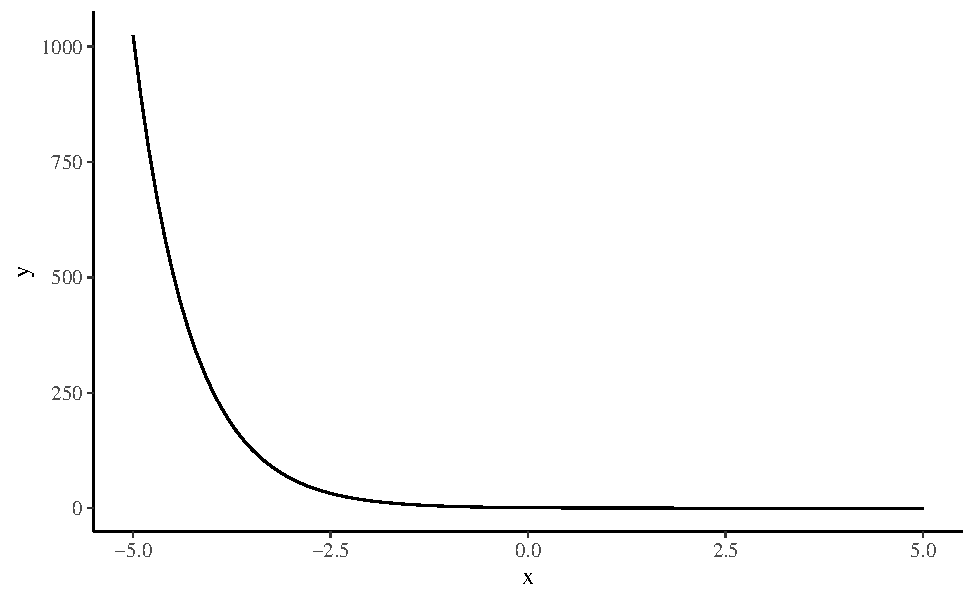
\includegraphics{ds4psy_files/figure-latex/unnamed-chunk-34-1} \end{center}

\hypertarget{quali-parametri-per-la-distribuzione-beta}{%
\subsection{Quali parametri per la distribuzione Beta?}\label{quali-parametri-per-la-distribuzione-beta}}

Se usiamo una distribuzione Beta per rappresentare le nostre credenze a priori sul parametro \(\theta\) (probabilità di successo), allora dobbiamo porci il problema di scegliere i parametri che definiscono la distribuzione Beta che meglio rappresenta le nostre opinioni a priori. Il modo più ovvio per ottenere questo risultato è per prove ed errori. Oppure, possiamo individuare i parametri \(\alpha\) e \(\beta\) della distribuzione interpretando \(\alpha\) come la nostra stima a priori del numero di ``successi'', \(\beta\) come a nostra stima a priori del numero di ``insuccessi'' e \(\alpha + \beta\) come il numero di prove del campione. Quindi, per esempio, se pensiamo che, su 30 prove, verranno osservati 10 successi, otteniamo una \(\mbox{Beta}(10, 20)\):

\begin{Shaded}
\begin{Highlighting}[]
\NormalTok{bayesrules}\SpecialCharTok{::}\FunctionTok{plot\_beta}\NormalTok{(}\DecValTok{10}\NormalTok{, }\DecValTok{20}\NormalTok{, }\AttributeTok{mean =} \ConstantTok{TRUE}\NormalTok{, }\AttributeTok{mode =} \ConstantTok{TRUE}\NormalTok{)}
\end{Highlighting}
\end{Shaded}

\begin{center}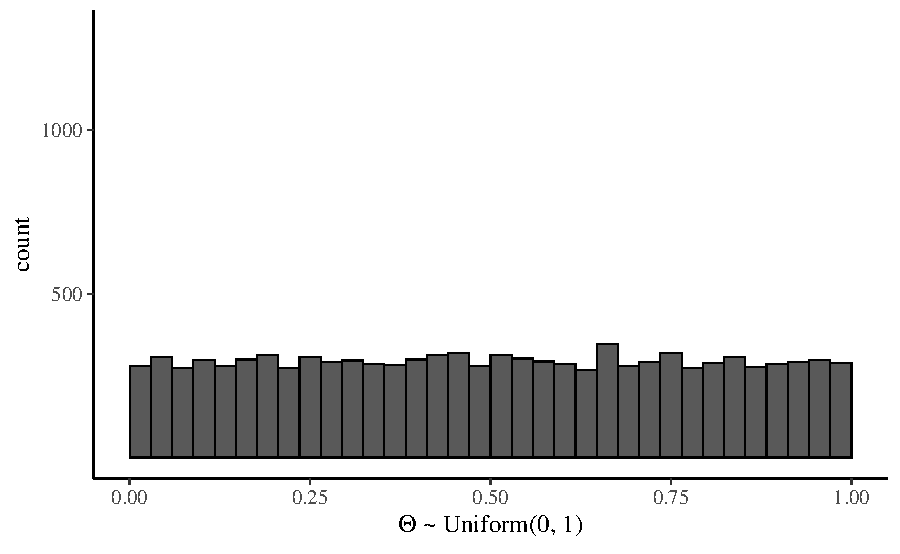
\includegraphics{ds4psy_files/figure-latex/unnamed-chunk-35-1} \end{center}

In alternativa, potremmo specificare la distribuzione a priori definendo la mediana e un quantile della distribuzione. Per esempio, le nostre opinioni a priori sul parametro potrebbero essere tali per cui pensiamo che la mediana della distribuzione sia 0.25 e il quantile della distribuzione di ordine 0.9 sia 0.5. Usando la Shiny App \texttt{ProbBayes::ChooseBeta()} troviamo i parametri \(\alpha = 1.84\) e \(\beta = 4.89\).

\hypertarget{commenti-e-considerazioni-finali-1}{%
\section*{Commenti e considerazioni finali}\label{commenti-e-considerazioni-finali-1}}


Abbiamo qui introdotto la procedura dell'aggiornamento bayesiano nel caso in cui la distribuzione a priori sia discreta. Abbiamo anche fornito alcune informazioni che sono utili per affrontare il problema nel caso in cui viene utilizzata una distribuzione a priori continua. Se viene utilizzata una distribuzione a priori continua, al denominatore del rapporto di Bayes troviamo un integrale che, in generale, non si può risolvere per via analitica. Il caso dell'inferenza di una proporzione, in cui la distribuzione a priori è una distribuzione Beta e la verosimiglianza è binoniale, rappresenta però un'eccezione, ovvero consente di derivare le proprietà della distribuzione a posteriori per via analitica. Il prossimo capitolo ha lo scopo di mostrare come questo possa essere fatto.

\hypertarget{chapter-distr-coniugate}{%
\chapter{Distribuzioni a priori coniugate}\label{chapter-distr-coniugate}}

Obiettivo di questo Capitolo è fornire un esempio di derivazione della distribuzione a posteriori scegliendo quale distribuzione a priori una distribuzione coniugata. Esamineremo qui il lo schema beta-binomiale.

\hypertarget{chapter-distr-priori-coniugate}{%
\section{Lo schema beta-binomiale}\label{chapter-distr-priori-coniugate}}

Iniziamo con una definizione.

\begin{definition}
Una distribuzione di probabilità a priori \(p(\theta)\) si dice \emph{coniugata} al modello usato se la distribuzione a priori e la distribuzione a posteriori hanno la stessa forma funzionale. Dunque, le due distribuzioni differiscono solo per il valore dei parametri.
\end{definition}

Ad esempio, se la distribuzione a priori è una distribuzione Beta e se la funzione di verosimiglianza è binomiale, allora anche la distribuzione a posteriori sarà una distribuzione Beta.

Da un punto di vista matematico, le distribuzioni a priori coniugate sono la scelta più conveniente in quanto ci consentono di calcolare analiticamente la distribuzione a posteriori con ``carta e penna'', senza la necessità di ricorrere a calcoli complessi. Da una prospettiva computazionale moderna, però, le distribuzioni a priori coniugate generalmente non sono migliori delle alternative, dato che i moderni metodi computazionali ci consentono di eseguire l'inferenza praticamente con qualsiasi scelta delle distribuzioni a priori, e non solo con le distribuzioni a priori che risultano matematicamente convenienti. Tuttavia, le famiglie coniugate offronto un utile ausilio didattico nello studio dell'inferenza bayesiana. Questo è il motivo per cui le esamineremo qui. Nello specifico, esamineremo quello che viene chiamato lo schema beta-binomiale.

Per fare un esempio concreto, consideriamo nuovamente i dati di \citet{zetschefuture2019}: nel campione di 30 partecipanti clinici le aspettative future di 23 partecipanti risultano negativamente distorte mentre quelle di 7 partecipanti risultano positivamente distorte. Nel seguito, indicheremo con \(\theta\) la probabilità che le aspettative di un paziente clinico siano distorte negativamente. Ci poniamo il problema di ottenere una stima a posteriori di \(\theta\) avendo osservato 23 ``successi'' in 30 prove.

I dati osservati (\(y = 23\)) possono essere considerati la manifestazione di una variabile casuale Bernoulliana. In tali circostanze, esiste una famiglia di distribuzioni che, qualora venga scelta per la distribuzione a priori, fa sì che la distribuzione a posteriori abbia la stessa forma funzionale della distribuzione a priori. Questo consente una soluzione analitica dell'integrale che compare a denominatore nella formula di Bayes. Nel caso presente, la famiglia di distribuzioni che ha questa proprietà è la distribuzione Beta.

\hypertarget{la-specificazione-della-distribuzione-a-priori}{%
\subsection{La specificazione della distribuzione a priori}\label{la-specificazione-della-distribuzione-a-priori}}

È possibile esprimere diverse credenze iniziali rispetto a \(\theta\) mediante la distribuzione Beta. Ad esempio, la scelta di una \(\mbox{Beta}(\alpha = 4, \beta = 4)\) quale distribuzione a priori per il parametro \(\theta\) corrisponde alla credenza a priori che associa all'evento ``presenza di una aspettativa futura distorta negativamente'' una grande incertezza: il valore 0.5 è il valore di \(\theta\) più plausibile, ma anche gli altri valori del parametro (tranne gli estremi) sono ritenuti piuttosto plausibili. Questa distribuzione a priori esprime la credenza che sia egualmente probabile per un'aspettativa futura essere distorta negativamente o positivamente.

\begin{Shaded}
\begin{Highlighting}[]
\FunctionTok{library}\NormalTok{(}\StringTok{"bayesrules"}\NormalTok{)}
\FunctionTok{plot\_beta}\NormalTok{(}\AttributeTok{alpha =} \DecValTok{4}\NormalTok{, }\AttributeTok{beta =} \DecValTok{4}\NormalTok{, }\AttributeTok{mean =} \ConstantTok{TRUE}\NormalTok{, }\AttributeTok{mode =} \ConstantTok{TRUE}\NormalTok{)}
\end{Highlighting}
\end{Shaded}

\begin{center}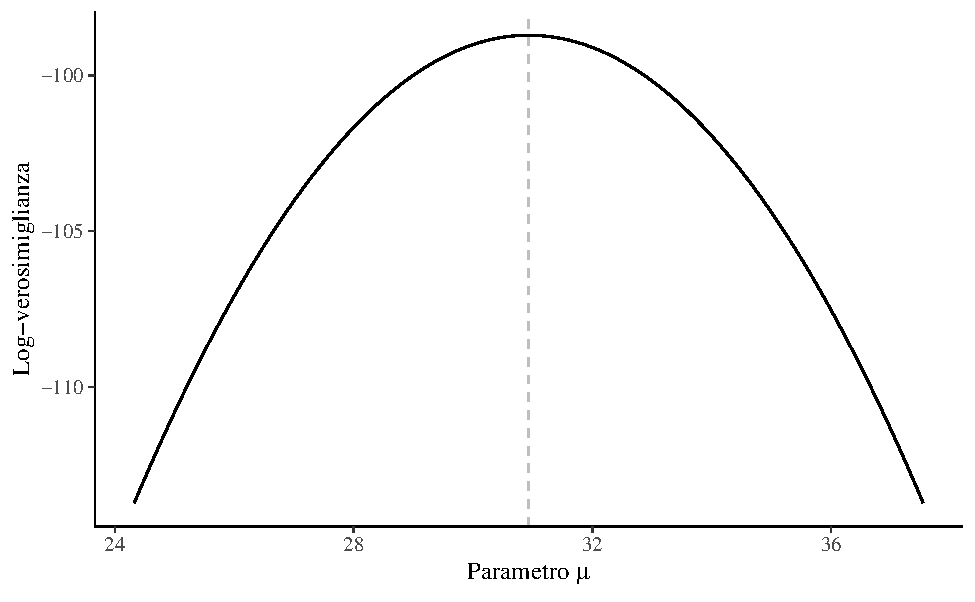
\includegraphics{ds4psy_files/figure-latex/unnamed-chunk-37-1} \end{center}

Possiamo quantificare la nostra incertezza calcolando, con un grado di fiducia del 95\%, la regione nella quale, in base a tale credenza a priori, si trova il valore del parametro. Per ottenere tale intervallo di credibilità a priori, usiamo la funzione \texttt{qbeta()} di \(\R\). In \texttt{qbeta()} i parametri \(\alpha\) e \(\beta\) sono chiamati \texttt{shape1} e \texttt{shape2}:

\begin{Shaded}
\begin{Highlighting}[]
\FunctionTok{qbeta}\NormalTok{(}\FunctionTok{c}\NormalTok{(}\FloatTok{0.025}\NormalTok{, }\FloatTok{0.975}\NormalTok{), }\AttributeTok{shape1 =} \DecValTok{4}\NormalTok{, }\AttributeTok{shape2 =} \DecValTok{4}\NormalTok{)}
\CommentTok{\#\textgreater{} [1] 0.1841 0.8159}
\end{Highlighting}
\end{Shaded}

Se poniamo \(\alpha=10\) e \(\beta=10\), questo corrisponde ad una credenza a priori che sia egualmente probabile per un'aspettativa futura essere distorta negativamente o positivamente,

\begin{Shaded}
\begin{Highlighting}[]
\FunctionTok{plot\_beta}\NormalTok{(}\AttributeTok{alpha =} \DecValTok{10}\NormalTok{, }\AttributeTok{beta =} \DecValTok{10}\NormalTok{, }\AttributeTok{mean =} \ConstantTok{TRUE}\NormalTok{, }\AttributeTok{mode =} \ConstantTok{TRUE}\NormalTok{)}
\end{Highlighting}
\end{Shaded}

\begin{center}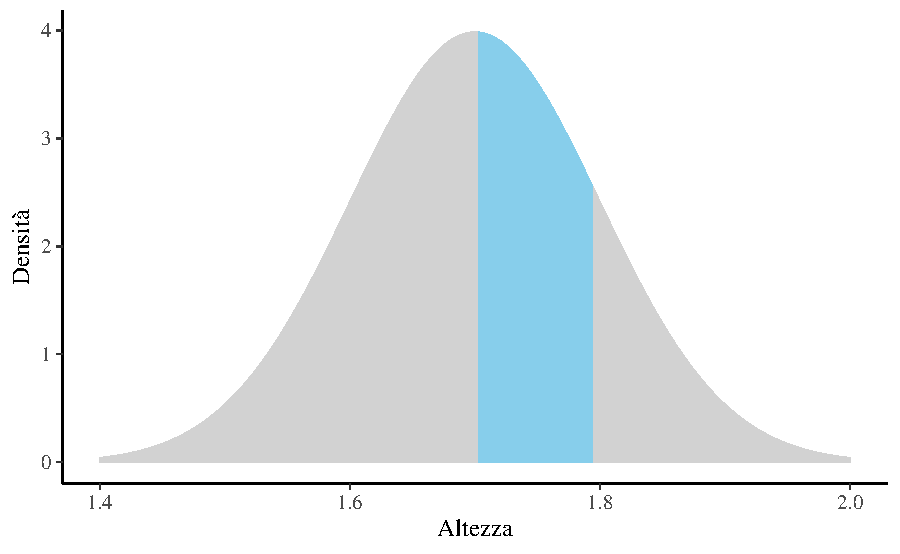
\includegraphics{ds4psy_files/figure-latex/unnamed-chunk-39-1} \end{center}

ma ora la nostra certezza a priori sul valore del parametro è maggiore, come indicato dall'intervallo al 95\%:

\begin{Shaded}
\begin{Highlighting}[]
\FunctionTok{qbeta}\NormalTok{(}\FunctionTok{c}\NormalTok{(}\FloatTok{0.025}\NormalTok{, }\FloatTok{0.975}\NormalTok{), }\AttributeTok{shape1 =} \DecValTok{10}\NormalTok{, }\AttributeTok{shape2 =} \DecValTok{10}\NormalTok{)}
\CommentTok{\#\textgreater{} [1] 0.2886 0.7114}
\end{Highlighting}
\end{Shaded}

Quale distribuzione a priori dobbiamo scegliere? In un problema concreto di analisi dei dati, la scelta della distribuzione a priori dipende dalle credenze a priori che vogliamo includere nell'analisi dei dati. Se non abbiamo alcuna informazione a priori, potremmo usare \(\alpha=1\) e \(\beta=1\), che produce una distribuzione a priori uniforme. Ma l'uso di distribuzioni a priori uniformi è sconsigliato per vari motivi, inclusa l'instabilità numerica della stima dei parametri. È meglio invece usare una distribuzione a priori debolmente informativa, come \(\mbox{Beta}(2, 2)\).

Nella discussione presente, solo per fare un esempio, useremo quale distribuzione a priori una \(\mbox{Beta}(2, 10)\), ovvero:

\[
p(\theta) = \frac{\Gamma(12)}{\Gamma(2)\Gamma(10)}\theta^{2-1} (1-\theta)^{10-1}.
\]

\begin{Shaded}
\begin{Highlighting}[]
\FunctionTok{plot\_beta}\NormalTok{(}\AttributeTok{alpha =} \DecValTok{2}\NormalTok{, }\AttributeTok{beta =} \DecValTok{10}\NormalTok{, }\AttributeTok{mean =} \ConstantTok{TRUE}\NormalTok{, }\AttributeTok{mode =} \ConstantTok{TRUE}\NormalTok{)}
\end{Highlighting}
\end{Shaded}

\begin{center}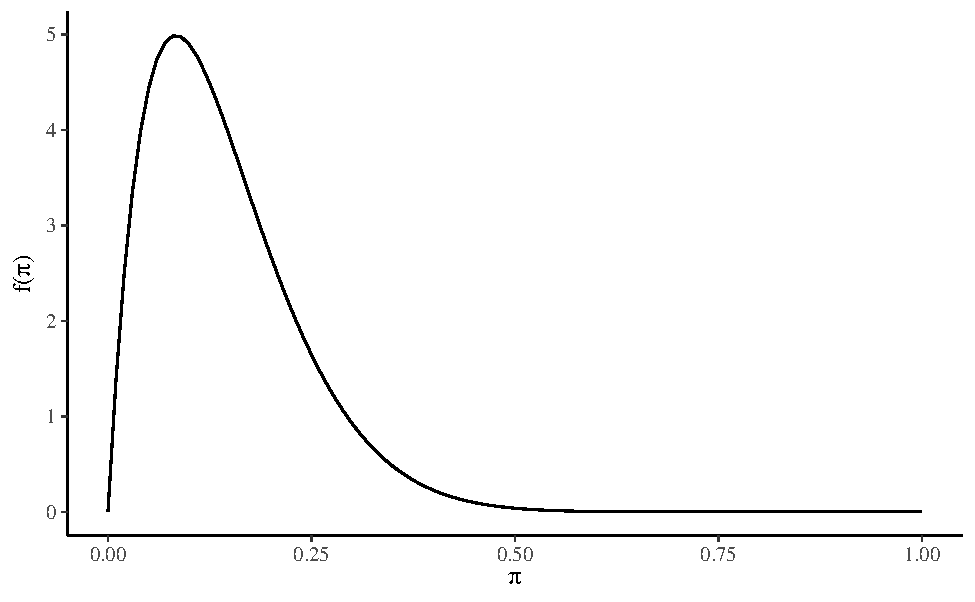
\includegraphics{ds4psy_files/figure-latex/unnamed-chunk-41-1} \end{center}

La \(\mbox{Beta}(2, 10)\) esprime la credenza che \(\theta < 0.5\), con il valore più plausibile pari a cicrca 0.1.

\hypertarget{la-specificazione-della-distribuzione-a-posteriori}{%
\subsection{La specificazione della distribuzione a posteriori}\label{la-specificazione-della-distribuzione-a-posteriori}}

Una volta scelta una distribuzione a priori di tipo Beta, i cui parametri rispecchiano le nostre credenze iniziali su \(\theta\), la distribuzione a posteriori viene specificata dalla formula di Bayes:

\[
\text{distribuzione a posteriori} = \frac{\text{verosimiglianza}\cdot\text{distribuzione a priori}}{\text{verosimiglianza marginale}}.
\]

Nel caso presente abbiamo

\[
p(\theta \mid n=30, y=23) = \frac{\Big[\binom{30}{23}\theta^{23}(1-\theta)^{30-23}\Big]\Big[\frac{\Gamma(12)}{\Gamma(2)\Gamma(10)}\theta^{2-1} (1-\theta)^{10-1}\Big]}{p(y = 23)},
\]

laddove \(p(y = 23)\), ovvero la verosimiglianza marginale, è una costante di normalizzazione.

Riscriviamo l'equazione precedente in termini più generali:

\[
p(\theta \mid n, y) = \frac{\Big[\binom{n}{y}\theta^{y}(1-\theta)^{n-y}\Big]\Big[\frac{\Gamma(a+b)}{\Gamma(a)\Gamma(b)}\theta^{a-1} (1-\theta)^{b-1}\Big]}{p(y)}
\]

Raccogliendo tutte le costanti otteniamo:

\[
p(\theta \mid n, y) =\left[\frac{\binom{n}{y}\frac{\Gamma(a+b)}{\Gamma(a)\Gamma(b)}}{p(y)}\right] \theta^{y}(1-\theta)^{n-y}\theta^{a-1} (1-\theta)^{b-1}.
\]

Se ignoriamo il termine costante all'interno della parentesi quadra

\begin{align}
p(\theta \mid n, y) &\propto \theta^{y}(1-\theta)^{n-y}\theta^{a-1} (1-\theta)^{b-1},\notag\\
&\propto \theta^{a+y-1}(1-\theta)^{b+n-y-1},\notag
\end{align}

il termine di destra dell'equazione precedente identifica il \emph{kernel} della distribuzione a posteriori e corrisponde ad una Beta \emph{non normalizzata} di parametri \(a + y\) e \(b + n - y\).

Per ottenere una distribuzione di densità, dobbiamo aggiungere una costante di normalizzazione al kernel della distribuzione a posteriori. In base alla definizione della distribuzione Beta, ed essendo \(a' = a+y\) e \(b' = b+n-y\), tale costante di normalizzazione sarà uguale a

\[
\frac{\Gamma(a'+b')}{\Gamma(a')\Gamma(b')} = \frac{\Gamma(a+b+n)}{\Gamma(a+y)\Gamma(b+n-y)}.
\]

In altri termini, nel caso dello schema beta-binomiale, la distribuzione a posteriori è una \(\mbox{Beta}(a+y, b+n-y)\):

\[
\mbox{Beta}(a+y, b+n-y) = \frac{\Gamma(a+b+n)}{\Gamma(a+y)\Gamma(b+n-y)} \theta^{a+y-1}(1-\theta)^{b+n-y-1}.
\]

In sintesi, moltiplicando verosimiglianza \(\mbox{Bin}(n = 30, y = 23 \mid \theta)\) per la la distribuzione a priori \(\theta \sim \mbox{Beta}(2, 10)\) e dividendo per la costante di normalizzazione, abbiamo ottenuto la distribuzione a posteriori \(p(\theta \mid n, y) \sim \mbox{Beta}(25, 17)\). Questo è un esempio di analisi coniugata. La presente combinazione di verosimiglianza e distribuzione a priori è chiamata caso coniugato \emph{beta-binomiale} ed è descritta dal seguente teorema.

\begin{theorem}
\protect\hypertarget{thm:post-beta-bin-1}{}\label{thm:post-beta-bin-1}Sia data la funzione di verosimiglianza \(\mbox{Bin}(n, y \mid \theta)\) e sia \(\mbox{Beta}(\alpha, \beta)\) una distribuzione a priori. In tali circostanze, la distribuzione a posteriori del parametro \(\theta\) sarà una distribuzione \(\mbox{Beta}(\alpha + y, \beta + n - y)\).
\end{theorem}

È facile calcolare il valore atteso a posteriori di \(\theta\). Essendo \(\E[\mbox{Beta}(\alpha, \beta)] = \frac{\alpha}{\alpha + \beta}\), il risultato cercato diventa

\begin{equation}
\E_{\text{post}} [\mathrm{Beta}(\alpha + y, \beta + n - y)] = \frac{\alpha + y}{\alpha + \beta +n}.
\label{eq:ev-post-beta-bin-1}
\end{equation}

\begin{exercise}

Si rappresenti in maniera grafica e si descriva in forma numerica l'aggiornamento bayesiano beta-binomiale per i dati di \citet{zetschefuture2019}. Si assuma una distribuzione a priori \(\mbox{Beta}(2, 10)\).

Per i dati in questione, l'aggiornamento bayesiano può essere rappresentato in forma grafica usando la funzione \texttt{plot\_beta\_binomial()} del pacchetto \texttt{bayesrules}:

\begin{Shaded}
\begin{Highlighting}[]
\NormalTok{bayesrules}\SpecialCharTok{::}\FunctionTok{plot\_beta\_binomial}\NormalTok{(}
  \AttributeTok{alpha =} \DecValTok{2}\NormalTok{, }\AttributeTok{beta =} \DecValTok{10}\NormalTok{, }\AttributeTok{y =} \DecValTok{23}\NormalTok{, }\AttributeTok{n =} \DecValTok{30}
\NormalTok{)}
\end{Highlighting}
\end{Shaded}

\begin{center}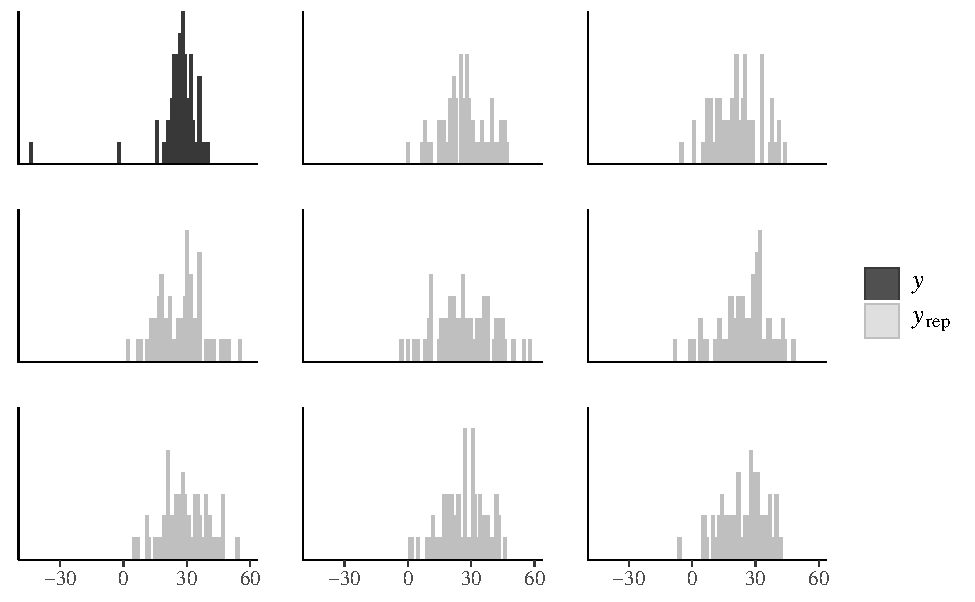
\includegraphics{ds4psy_files/figure-latex/unnamed-chunk-42-1} \end{center}

Oppure, possiamo scrivere noi stessi una funzione, come ad esempio la funzione \texttt{plot\_beta\_binom()} riportata in Appendice \ref{appendix:beta-binom}. Mediante tale la funzione otteniamo

\begin{Shaded}
\begin{Highlighting}[]
\FunctionTok{plot\_beta\_bin}\NormalTok{(}\DecValTok{2}\NormalTok{, }\DecValTok{10}\NormalTok{, }\DecValTok{23}\NormalTok{, }\DecValTok{30}\NormalTok{)}
\end{Highlighting}
\end{Shaded}

\begin{center}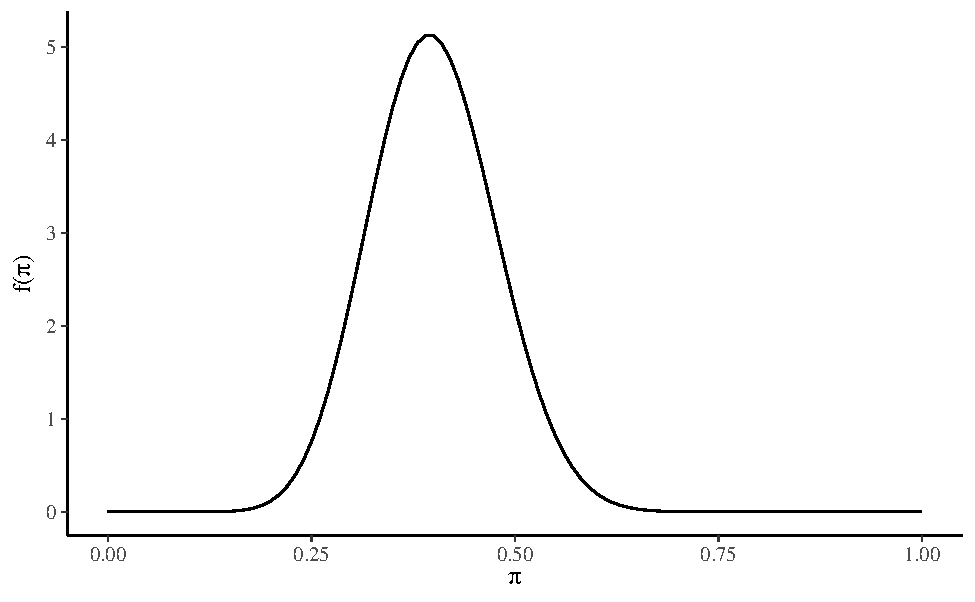
\includegraphics{ds4psy_files/figure-latex/unnamed-chunk-44-1} \end{center}

Un sommario delle distribuzioni a priori e a posteriori può essere ottenuto, ad esempio, usando la funzione \texttt{summarize\_beta\_binomial()} del pacchetto \texttt{bayesrules}:

\begin{Shaded}
\begin{Highlighting}[]
\NormalTok{bayesrules}\SpecialCharTok{:::}\FunctionTok{summarize\_beta\_binomial}\NormalTok{(}
  \AttributeTok{alpha =} \DecValTok{2}\NormalTok{, }\AttributeTok{beta =} \DecValTok{10}\NormalTok{, }\AttributeTok{y =} \DecValTok{23}\NormalTok{, }\AttributeTok{n =} \DecValTok{30}
\NormalTok{)}
\CommentTok{\#\textgreater{}       model alpha beta   mean mode      var      sd}
\CommentTok{\#\textgreater{} 1     prior     2   10 0.1667  0.1 0.010684 0.10336}
\CommentTok{\#\textgreater{} 2 posterior    25   17 0.5952  0.6 0.005603 0.07485}
\end{Highlighting}
\end{Shaded}

\end{exercise}

\begin{exercise}

Per i dati di \citet{zetschefuture2019}, si trovino la media, la moda, la deviazione standard della distribuzione a posteriori di \(\theta\). Si trovi inoltre l'intervallo di credibilità a posteriori del 95\% per il parametro \(\theta\).

Usando il Teorema \ref{thm:post-beta-bin-1}, l'intervallo di credibilità a posteriori del 95\% per il parametro \(\theta\) è:

\begin{Shaded}
\begin{Highlighting}[]
\FunctionTok{qbeta}\NormalTok{(}\FunctionTok{c}\NormalTok{(}\FloatTok{0.025}\NormalTok{, }\FloatTok{0.975}\NormalTok{), }\AttributeTok{shape1 =} \DecValTok{25}\NormalTok{, }\AttributeTok{shape2 =} \DecValTok{17}\NormalTok{)}
\CommentTok{\#\textgreater{} [1] 0.4450 0.7368}
\end{Highlighting}
\end{Shaded}

Usando la \eqref{eq:ev-post-beta-bin-1}, la media della distribuzione a posteriori è

\begin{Shaded}
\begin{Highlighting}[]
\DecValTok{25} \SpecialCharTok{/}\NormalTok{ (}\DecValTok{25} \SpecialCharTok{+} \DecValTok{17}\NormalTok{)}
\CommentTok{\#\textgreater{} [1] 0.5952}
\end{Highlighting}
\end{Shaded}

Per le proprietà della distribuzione Beta, la moda della distribuzione a posteriori è

\begin{Shaded}
\begin{Highlighting}[]
\NormalTok{(}\DecValTok{25} \SpecialCharTok{{-}} \DecValTok{1}\NormalTok{) }\SpecialCharTok{/}\NormalTok{ (}\DecValTok{25} \SpecialCharTok{+} \DecValTok{17} \SpecialCharTok{{-}} \DecValTok{2}\NormalTok{)}
\CommentTok{\#\textgreater{} [1] 0.6}
\end{Highlighting}
\end{Shaded}

e la deviazione standard della distribuzione a priori è

\begin{Shaded}
\begin{Highlighting}[]
\FunctionTok{sqrt}\NormalTok{((}\DecValTok{25} \SpecialCharTok{*} \DecValTok{17}\NormalTok{) }\SpecialCharTok{/}\NormalTok{ ((}\DecValTok{25} \SpecialCharTok{+} \DecValTok{17}\NormalTok{)}\SpecialCharTok{\^{}}\DecValTok{2} \SpecialCharTok{*}\NormalTok{ (}\DecValTok{25} \SpecialCharTok{+} \DecValTok{17} \SpecialCharTok{+} \DecValTok{1}\NormalTok{)))}
\CommentTok{\#\textgreater{} [1] 0.07485}
\end{Highlighting}
\end{Shaded}

\end{exercise}

\begin{exercise}

Si trovino i parametri e le proprietà della distribuzione a posteriori del parametro \(\theta\) per i dati dell'esempio relativo alla ricerca di Stanley Milgram discussa da \citet{Johnson2022bayesrules}.

Nel 1963, Stanley Milgram presentò una ricerca sulla propensione delle persone a obbedire agli ordini di figure di autorità, anche quando tali ordini possono danneggiare altre persone \citep{milgram1963behavioral}. Nell'articolo, Milgram descrive lo studio come \emph{``consist{[}ing{]} of ordering a naive subject to administer electric shock to a victim. A simulated shock generator is used, with 30 clearly marked voltage levels that range from IS to 450 volts. The instrument bears verbal designations that range from Slight Shock to Danger: Severe Shock. The responses of the victim, who is a trained confederate of the experimenter, are standardized. The orders to administer shocks are given to the naive subject in the context of a `learning experiment' ostensibly set up to study the effects of punishment on memory. As the experiment proceeds the naive subject is commanded to administer increasingly more intense shocks to the victim, even to the point of reaching the level marked Danger: Severe Shock.''}

All'insaputa del partecipante, gli shock elettrici erano falsi e l'attore stava solo fingendo di provare il dolore dello shock.

\citet{Johnson2022bayesrules} fanno inferenza sui risultati dello studio di Milgram mediante il modello Beta-Binomiale. Il parametro di interesse è \(\theta\), la probabiltà che una persona obbedisca all'autorità (in questo caso, somministrando lo shock più severo), anche se ciò significa recare danno ad altri. \citet{Johnson2022bayesrules} ipotizzano che, prima di raccogliere dati, le credenze di Milgram relative a \(\theta\) possano essere rappresentate mediante una \(\mbox{Beta}(1, 10)\). Sia \(y = 26\) il numero di soggetti che, sui 40 partecipanti allo studio, aveva accettato di infliggere lo shock più severo. Assumendo che ogni partecipante si comporti indipendentemente dagli altri, possiamo modellare la dipendenza di \(y\) da \(\theta\) usando la distribuzione binomiale. Giungiamo dunque al seguente modello bayesiano Beta-Binomiale:

\begin{align}
y \mid \theta & \sim \mbox{Bin}(n = 40, \theta) \notag\\
\theta & \sim \text{Beta}(1, 10) \; . \notag
\end{align}

Usando le funzioni di \texttt{bayesrules} possiamo facilmente calcolare i parametri e le proprietà della distribuzione a posteriori:

\begin{Shaded}
\begin{Highlighting}[]
\NormalTok{bayesrules}\SpecialCharTok{:::}\FunctionTok{summarize\_beta\_binomial}\NormalTok{(}
  \AttributeTok{alpha =} \DecValTok{1}\NormalTok{, }\AttributeTok{beta =} \DecValTok{10}\NormalTok{, }\AttributeTok{y =} \DecValTok{26}\NormalTok{, }\AttributeTok{n =} \DecValTok{40}
\NormalTok{)}
\CommentTok{\#\textgreater{}       model alpha beta    mean   mode      var      sd}
\CommentTok{\#\textgreater{} 1     prior     1   10 0.09091 0.0000 0.006887 0.08299}
\CommentTok{\#\textgreater{} 2 posterior    27   24 0.52941 0.5306 0.004791 0.06922}
\end{Highlighting}
\end{Shaded}

Il processo di aggiornamento bayesiano è descritto dalla figura seguente:

\begin{Shaded}
\begin{Highlighting}[]
\FunctionTok{plot\_beta\_bin}\NormalTok{(}\DecValTok{1}\NormalTok{, }\DecValTok{10}\NormalTok{, }\DecValTok{26}\NormalTok{, }\DecValTok{40}\NormalTok{)}
\end{Highlighting}
\end{Shaded}

\begin{center}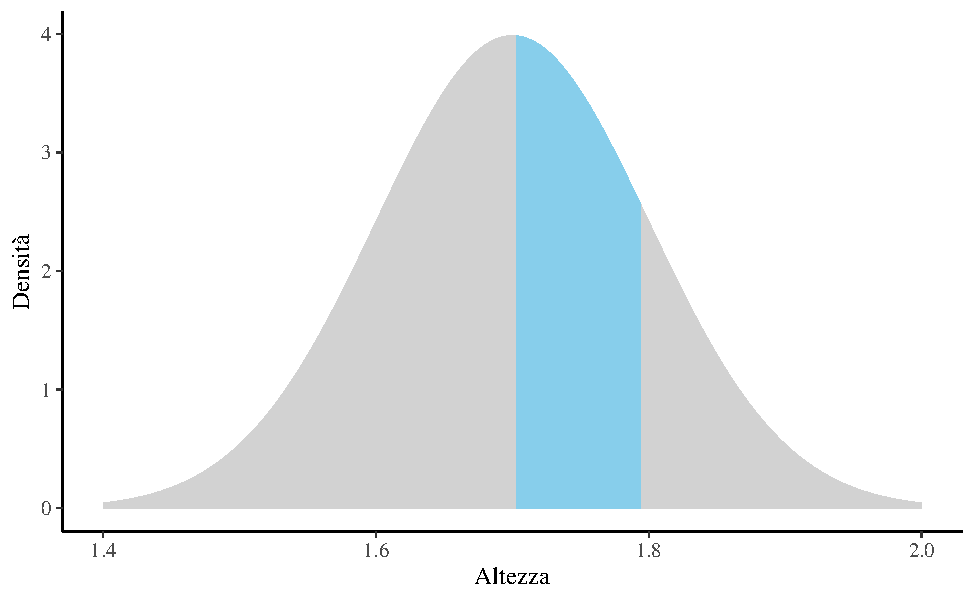
\includegraphics{ds4psy_files/figure-latex/unnamed-chunk-51-1} \end{center}

\end{exercise}

\hypertarget{inferenza-bayesiana-con-distribuzioni-a-priori-continue}{%
\section{Inferenza bayesiana con distribuzioni a priori continue}\label{inferenza-bayesiana-con-distribuzioni-a-priori-continue}}

L'inferenza bayesiane sulla proporzione \(\pi\) si basa su vari riepiloghi della distribuzione a posteriori Beta. Il riepilogo che si calcola dalla distribuzione a posteriori dipende dal tipo di inferenza. Consideriamo qui su due tipi di inferenza: (1) problemi in cui si è interessati a valutare la plausibilità che il parametro assuma valori contenuti in un dato intervallo di valori, (2) stime dell'intervallo che contiene il parametro ad un dato livello di probabilità soggettiva.

\hypertarget{approccio-bayesiano-alla-verifica-di-ipotesi}{%
\subsection{Approccio bayesiano alla verifica di ipotesi}\label{approccio-bayesiano-alla-verifica-di-ipotesi}}

Nell'esempio precedente sui dati di \citet{zetschefuture2019}, la nostra credenza a posteriori relativa a \(\theta\) (probabilità che l'aspettativa dell'umore futuro sia distorta negativamente) è descritta da una distribuzione Beta(25,17). Una volta definita la distribuzione a posteriori, ci possiamo porre altre domande. Per esempio: qual è la probabilità che \(\theta\) sia maggiore di 0.5?

Una risposta a questa domanda si trova con

\begin{Shaded}
\begin{Highlighting}[]
\DecValTok{1} \SpecialCharTok{{-}} \FunctionTok{pbeta}\NormalTok{(}\FloatTok{0.5}\NormalTok{, }\DecValTok{25}\NormalTok{, }\DecValTok{17}\NormalTok{)}
\CommentTok{\#\textgreater{} [1] 0.8945}
\end{Highlighting}
\end{Shaded}

oppure, in maniera equivalente, con

\begin{Shaded}
\begin{Highlighting}[]
\NormalTok{ProbBayes}\SpecialCharTok{::}\FunctionTok{beta\_area}\NormalTok{(}\AttributeTok{lo =} \FloatTok{0.5}\NormalTok{, }\AttributeTok{hi =} \FloatTok{1.0}\NormalTok{, }\AttributeTok{shape\_par =} \FunctionTok{c}\NormalTok{(}\DecValTok{25}\NormalTok{, }\DecValTok{17}\NormalTok{))}
\end{Highlighting}
\end{Shaded}

\begin{center}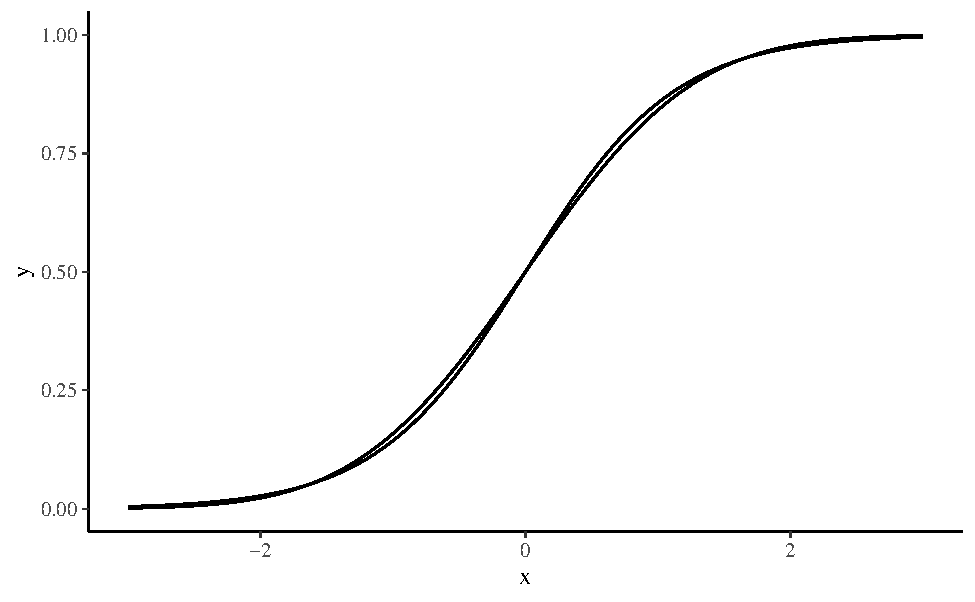
\includegraphics{ds4psy_files/figure-latex/unnamed-chunk-53-1} \end{center}

Questo calcolo può essere svolto mediante simulazione. Dato che conosciamo la distribuzione target, è possibile ricavare un campione casuale di osservazioni da una tale distribuzione e poi riassumere il campione in modo da calcolare \(\theta > 0.5\).

\begin{Shaded}
\begin{Highlighting}[]
\NormalTok{nsim }\OtherTok{\textless{}{-}} \FloatTok{1e6}
\NormalTok{theta\_samples }\OtherTok{\textless{}{-}} \FunctionTok{rbeta}\NormalTok{(nsim, }\DecValTok{25}\NormalTok{, }\DecValTok{17}\NormalTok{)}
\FunctionTok{sum}\NormalTok{(theta\_samples }\SpecialCharTok{\textgreater{}} \FloatTok{0.5}\NormalTok{) }\SpecialCharTok{/}\NormalTok{ nsim}
\CommentTok{\#\textgreater{} [1] 0.8943}
\end{Highlighting}
\end{Shaded}

Il risultato della simulazione è molto simile a quello ottenuto in precedenza.

\hypertarget{intervalli-di-credibilituxe0}{%
\subsection{Intervalli di credibilità}\label{intervalli-di-credibilituxe0}}

Un secondo tipo di inferenza bayesiana è quella che ci porta a formulare gli intervalli di credibilità. Un intervallo di credibilità di ordine \(a \in [0, 1]\) è l'intervallo di valori che contiene una proporzione della distribuzione a posteriori pari ad \(a\). La funzione \texttt{ProbBayes::beta\_interval()} consente di calcolare l'intervallo di credibilità che lascia la stessa probabilità nelle due code. Per esempio, l'intervallo di credibilità all'89\% per la distribuzione a posteriori dell'esempio relativo ai dati di \citet{zetschefuture2019} è

\begin{Shaded}
\begin{Highlighting}[]
\NormalTok{ProbBayes}\SpecialCharTok{::}\FunctionTok{beta\_interval}\NormalTok{(}\FloatTok{0.89}\NormalTok{, }\FunctionTok{c}\NormalTok{(}\DecValTok{25}\NormalTok{, }\DecValTok{17}\NormalTok{))}
\end{Highlighting}
\end{Shaded}

\begin{center}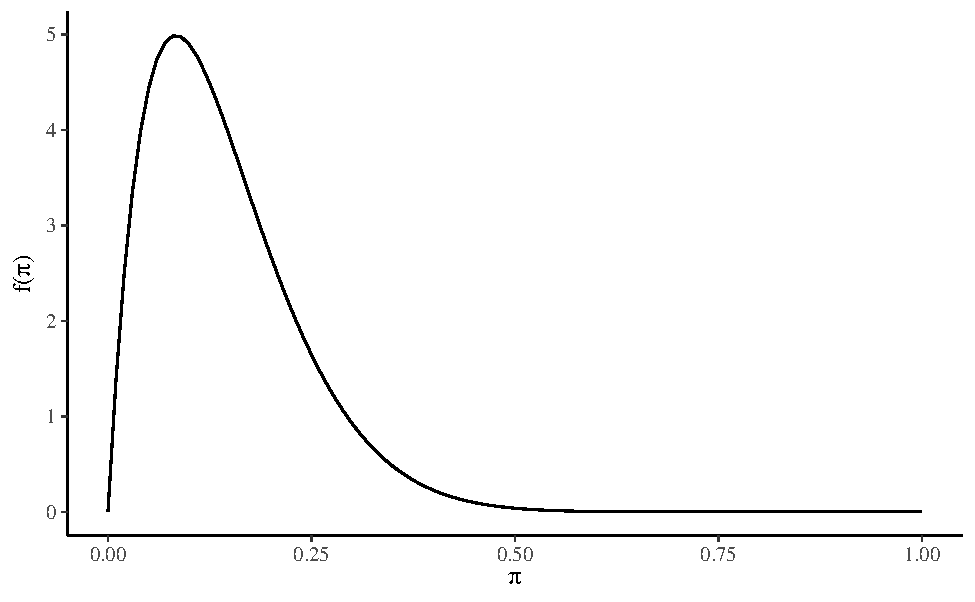
\includegraphics{ds4psy_files/figure-latex/unnamed-chunk-55-1} \end{center}

L'intervallo di credibilità all'50\% per la distribuzione a posteriori dell'esempio relativo ai dati di \citet{zetschefuture2019} è

\begin{Shaded}
\begin{Highlighting}[]
\NormalTok{ProbBayes}\SpecialCharTok{::}\FunctionTok{beta\_interval}\NormalTok{(}\FloatTok{0.5}\NormalTok{, }\FunctionTok{c}\NormalTok{(}\DecValTok{25}\NormalTok{, }\DecValTok{17}\NormalTok{))}
\end{Highlighting}
\end{Shaded}

\begin{center}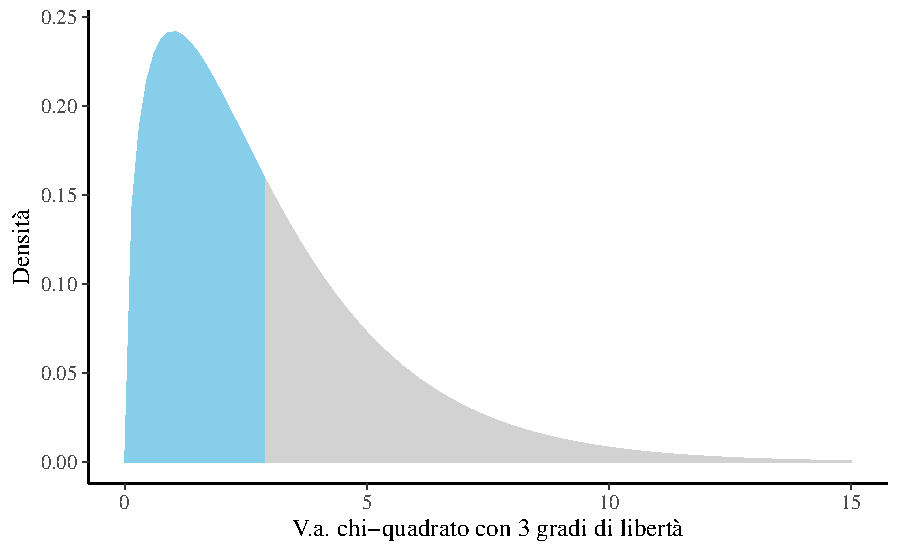
\includegraphics{ds4psy_files/figure-latex/unnamed-chunk-56-1} \end{center}

\hypertarget{principali-distribuzioni-coniugate}{%
\section{Principali distribuzioni coniugate}\label{principali-distribuzioni-coniugate}}

Esistono molte altre combinazioni simili di verosimiglianza e distribuzione a priori le quali producono una distribuzione a posteriori che ha la stessa densità della distribuzione a priori. Sono elencate qui sotto le più note coniugazioni tra modelli statistici e distribuzioni a priori.

\begin{itemize}
\tightlist
\item
  Per il modello Normale-Normale \(\mathcal{N}(\mu, \sigma^2_0)\), la distribizione iniziale è \(\mathcal{N}(\mu_0, \tau^2)\) e la distribuzione finale è \(\mathcal{N}\left(\frac{\mu_0\sigma^2 + \bar{y}n\tau^2}{\sigma^2 + n\tau^2}, \frac{\sigma^2\tau^2}{\sigma^2 + n\tau^2} \right)\).
\item
  Per il modello Poisson-gamma \(\text{Po}(\theta)\), la distribizione iniziale è \(\Gamma(\lambda, \delta)\) e la distribuzione finale è \(\Gamma(\lambda + n \bar{y}, \delta +n)\).
\item
  Per il modello esponenziale \(\text{Exp}(\theta)\), la distribizione iniziale è \(\Gamma(\lambda, \delta)\) e la distribuzione finale è \(\Gamma(\lambda + n, \delta +n\bar{y})\).
\item
  Per il modello uniforme-Pareto \(\text{U}(0, \theta)\), la distribizione iniziale è \(\mbox{Pa}(\alpha, \varepsilon)\) e la distribuzione finale è \(\mbox{Pa}(\alpha + n, \max(y_{(n)}, \varepsilon))\).
\end{itemize}

\hypertarget{commenti-e-considerazioni-finali-2}{%
\section*{Commenti e considerazioni finali}\label{commenti-e-considerazioni-finali-2}}


Lo scopo di questa discussione è mostrare come sia possibile combinare le nostre conoscenze a priori (espresse nei termini di una densità di probabilità) con le evidenze fornite dai dati (espresse nei termini della funzione di verosimiglianza), così da determinare, mediante il teorema di Bayes, una distribuzione a posteriori, la quale condensa l'incertezza che abbiamo sul parametro \(\theta\). Per illustrare tale problema, abbiamo considerato una situazione nella quale \(\theta\) corrisponde alla probabilità di successo in una sequenza di prove Bernoulliane. In tali circostanze è ragionevole esprimere le nostre credenze a priori mediante la densità Beta, con opportuni parametri. L'inferenza rispetto a \(\theta\) può essere svolta utilizzando una distribuzione a priori Beta e una verosimiglianza binomiale. Così facendo, la distribuzione a posteriori diventa essa stessa una distribuzione Beta -- questo è il cosiddetto schema beta-binomiale. Dato che utilizza una distribuzione a priori coniugata, lo schema beta-binomiale rende possibile la determinazione analitica dei parametri della distribuzione a posteriori.

  \bibliography{refs.bib,book.bib,packages.bib}

\printindex

\end{document}
